%%This is the KMD un-official thesis template (Engineering Format for English Writer).

\documentclass[12pt]{report}
\usepackage{kmd-emthesis}
\usepackage{graphicx}
\usepackage{subfigure}
\usepackage{tabularx}
\usepackage{longtable}
\usepackage{multirow}
\usepackage{url}
\usepackage{fancybox}
\usepackage{amssymb}
\usepackage{moreverb}
\usepackage{afterpage}
\usepackage{cite}
%\usepackage{harvard-oikos}
\usepackage{ccaption} % caption
\usepackage{fn2end} %footnotes script
\usepackage{fn2end_config} %footnotes edit script
\usepackage{indentfirst}
\usepackage{float}
\usepackage{listings}
\usepackage{amsmath}
\lstset{
  basicstyle=\small\ttfamily,
  columns=flexible,
  breaklines=true
}
\usepackage{booktabs}
%%%%%%%%%%%%%%%%%%%%%%%%%%%%

\makeatother

% Page Style Settings
\pagestyle{final}       % Final Draft
%\pagestyle{draft}      % Drafts

% Language Settings
\lang{English} % English

% Student ID number
\studentnumber{71744696}

% Choosing Masters Thesis or Report
\doctitle{\bachelorsreport}

% What Degree to obtain
\major{\envandinfo}

% Title (in LaTeX)
\etitle{Modeling Head-Bobbing in Pigeon Locomotion using Reinforcement Learning}

% Title (in plain text)
%   No need to set if the same as  (in LaTeX)
\eptitle{Practice of Design Thinking Workshop to Develop ``Media Innovator'' Leading Creative Society}


%Author's Name (in LaTeX)
\eauthor{Mioto Takahashi}

% Author's Name (in plain text)
%   No need to set if the same as in (in LaTeX)
% \epauthor{Mioto Takahashi}


% Academic Year
\syear{2022}
%\heiseiyear{24}
%\smonth{2}
%\sday{7}


% Advisors
\ecomembers{Professor Tatsuya Hagino}{(Supervisor)}
           {Professor Takashi Hattori}{(Co-Supervisor)}
           {}{}
           {}{}
\eaddcomembers{}{}

% 5 or 6 Keywords (in LaTeX)
\ekeywords{Reinforcement Learning, Biomimetic, Pigeon, Locomotion}

% 5 or 6 Keywords (in plain text)
% \epkeywords{Design Thinking, Creative Society, Workshop, Innovation, Education}

%Choose one submission category from [Design, Science / Engineering, Social Science / Humanities, Action Research]
\ecategory{Science / Engineering}
%Choose one submission category from [Design, Science / Engineering, Social Science / Humanities, Action Research] (in plain text)
% \ecategory{Science / Engineering}


%%%%%%%%%%%%%%%%%%%%%%%%%%Abstract%%%%%%%%%%%%%%%%%%%%%%%%%%%%%%%%%
\eabstract{

Lorem ipsum dolor sit amet, consectetur adipiscing elit. In efficitur porta augue, at interdum nunc lobortis at. Morbi feugiat facilisis justo, vitae maximus dolor. Cras convallis at elit in porta. Fusce lobortis tortor nibh, quis imperdiet arcu luctus quis. Mauris imperdiet urna eu mauris aliquet, vitae tincidunt orci dapibus. Vestibulum convallis elit ut velit accumsan cursus. Pellentesque lacus lacus, blandit eu felis vitae, pellentesque dignissim est.
}
%%%%%%%%%%%%%%%%%%%%%%%%% Document starts here %%%%%%%%%%%%%%%%%%%%%%%%%%%%


\begin{document}
  \titlepage
  \comemberspage
  \firstabstract
  %\secondabstract

  % Table of Contents
  \toc
  \newpage
  \listoffigures
  %\listoftables


  \newpage
  \pagenumbering{arabic}
  % Chapters
  \chapter{Background: Reinforcement Learning} \label{ch:background}
% \section{Reinforcement Learning}
% rl feedback loop and reward system
  Reinforcement learning is a type of control system that attempts to execute tasks described by manually set cost functions by minimizing them using optimization algorithms or learning algorithms. In the case of deep reinforcement learning, the controller is modeled using deep neural networks and the cost function is minimized using gradient descent algorithms.

  Reinforcement learning divides control systems into an agent and an environment. The agent acts the controller of the system that inspects its environment's state and sends output signals, or actions, that affect the environment. This mutual interactions creates a feedback loop between the two modules.

  In the context of a pigeon tasked to move forward, the pigeon's brain and its nervous system connected to each limb act as the agent, and its surroundings, such as the ground and arbitrary objects on it, act as the environment. The environment outputs a state, such as the global position of the pigeon, which is used as the input for the agent. Using the provided state, the agent calculates and outputs an action, such as the torque of each joint in the pigeon's body. The action alters the state of the environment, and the environment outputs a new state and a reward. The reward describes how well the pigeon was able to execute its task, such as the current position of the pigeon relative to its previous timestep. The agent is updated to output sequences of actions that maximizes the cumulative reward, or return. The return can be interpreted as the inverted or negated cost function.

% using reward as a cost function / constraint / task def
  Deep reinforcement learning algorithms can train deep neural network controllers to maximize cumulative sums of arbitrarily-defined reward functions, as long as they are achievable within the given environment. Therefore, in application to biology, we can encode constraints and definitions of tasks, such as behaviors produced by biological organisms, into reward functions, train control systems to follow such constraints and tasks, and generate behaviors accordingly, while abiding by the laws of physics.

% drl examples
  Notable deep reinforcement learning algorithms include proximal policy optimization (PPO) \cite{schulman2017proximal} and soft actor critic (SAC) \cite{haarnoja2018soft}.
  PPO is used as baseline for many reinforcement learning experiments such as building agents to play games, particularly Pommerman \cite{gao2019skynet}, controlling automated vehicles \cite{guan2020centralized}, and controlling unmanned aircrafts \cite{bohn2019deep}.
  On the other hand, SAC has been shown to perform better than PPO in benchmark tests and has been applied to biology-inspired robotics, particularly quadrupedal robotic control \cite{haarnoja2018softappli}.

  \section{Preliminary Research}
\subsection{Modeling biological phenomena}
% Robotics and Animals paper
  % Discusses pros and limitations of robotics as biological modeling
  % Algorithmic model vs Robotic model
    % Algorithmic models inferior to robotic models
    % Where can we use algorithmic models
    % Connect to this pigeon research
  % Learning model uses
    % Examples
    % Tie into current research
  % Incremental models
    % Method to tackle discrepancies between complexity of biological phenomena and its model
    % Tie into current research

\subsection{Head-Bobbing in Pigeons}
% Head-bobbing = Head stabilization
  % The "head-bob" behavior in pigeons consists of stabilizing the location and orientation of the head and altering them periodically. Such are dubbed as the hold phase and the thrust phase, respectively \cite{frost_1978}.
% Head stabilization used for stabilizing vision
  % Mainly 2 hypothesis regarding the functionalities of such behavior have been proposed \cite{frost_1978} \cite{davies_1988}.
  Both hypothesis suggest that the hold phase is utilized for stabilizing vision.
% Introduce 2 Hypothesis
% How each of the 2 hypothesis diverge
  % What this explains
  % What the shortcomings are
% Side note: 2 more hypothesis mentioned in the two papers that we are probably going to ignore

  \chapter{Approach}
Our research purpose is to verify whether preliminary hypotheses regarding the functionalities of head-bobbing, particularly visual stabilization and motion parallax, are sufficient to cause such behavior. We would like to examine whether there are possibilities of other causes or functionalities that may contribute to generating such particular movements.

% def of pigeon model
\section{Definition of the Pigeon Model}
  We define a simplified 2-dimensional model of pigeons based on incremental modeling. The pigeon model consists of 3 joints connecting one body representing the head, 2 bodies representing the neck, and one body representing the torso. The model's physics, mainly the collision and gravity, is simulated in a 2 dimensional physics engine. The torso's orientation and y-position is fixed while its x-position is incremented by a constant value. This represents forward locomotion at a constant speed.

  Additionally, we build control systems for the model using deep reinforcement learning. By using deep reinforcement learning, we can train the controller to maximize reward functions that represent hypotheses or manually-defined trajectories for the bodies in the model to follow.

\section{Baseline: Manually-Defined Head Trajectory}
  As the baseline for the model's control system, we attempt to recreate the head-bob movement by setting a target position for the head's position to match every timestep. The target position is first defined at a set location in front of the pigeon model $T$ relative to the position of its torso. The target then acts as a static position in the global coordinate for the head to follow. If the distance between the target position and the torso's position goes below a set threshold value, the target is repositioned at the same location $T$ relative to the torso's position.

\section{Hypothesis Testing}
  For verifying the preliminary hypotheses we compare the behaviors of the pigeon model produced by the baseline control system to those generated by the control system that represents preliminary hypotheses.

  %% description below should assume that we already know the angle of objects within retina
  Preliminary hypotheses for the functionalities of head-bobbing behavior can be depicted using two reward functions, each representing head stabilization ${r_{head\_stabilize}}$ and motion parallax ${r_{motion\_parallax}}$.

  The reward function that represents the hypothesis is described as below.
  \begin{equation}
    {r_{fifty\_fifty}}_t = {r_{head\_stabilize}}_t + {r_{motion\_parallax}}_t
  \end{equation}
  where $r_t$ is the reward at timestep $t$.

  % Hold phase: Head stabilization
  \subsection{Head Stabilization}
    Davies' hypothesis indicate that static objects should be stabilized into one location in the retina for the pigeon to easily determine the moving objects' velocities during the hold phase. In application, the pigeon's head should move in a trajectory that minimizes retinal velocities of objects.

    We define the reward function for head stabilization as,
    \begin{equation}
      {r_{head\_stabilize}}_t = - \sum_i^n |\dot {\theta_i}_t|
    \end{equation}
    where $n$ is the number of objects in the environment and $\dot \theta$ is the angular velocity of each object.

  % Thrust phase: Maximizing motion parallax
  \subsection{Motion Parallax}
    Frost and Davies's hypotheses indicate that differences in distances between objects from the pigeon's retina can be emphasized by inducing motion parallax.
    The sum of angular velocities of objects relative to each other should be maximized.

    We define the reward function for motion parallax as follows.
    \begin{equation}
      {r_{motion\_parallax}}_t = \sum_i^n \sum_{j \ne i}^n |\dot {\theta_i}_t - \dot {\theta_j}_t|
    \end{equation}


\section{Notable Questions}
  Given our approach, we can see that combining the reward functions for head stabilization and motion parallax result in a tradeoff between having to lock the position of the head in one place and having to move the head around. Therefore, it is of our belief that two more questions need to be addressed:

  \begin{itemize}
    \item Can hold and thrust phases emerge if given such tradeoff?
    \begin{description}
      \item
    \end{description}

    \item How would optimization algorithms solve this tradeoff?
    \begin{description}
      \item
    \end{description}
  \end{itemize}

  \chapter{Experiments} \label{ch:experiments}
We compare the trajectories of the bodies in the baseline control systems to those generated by control systems that represent preliminary hypotheses. By examining the similarities and differences between the trajectories, we can verify whether the preliminary hypotheses are sufficient for producing the head-bobbing behaviors seen in pigeons.

\section{Dimensions of the Pigeon Model}
  Our pigeon model's dimensions and orientations are set at static values for all experiments, as shown in Figure \ref{fig:pigeon_dimension}.
    \begin{figure}[H]
        \centering
        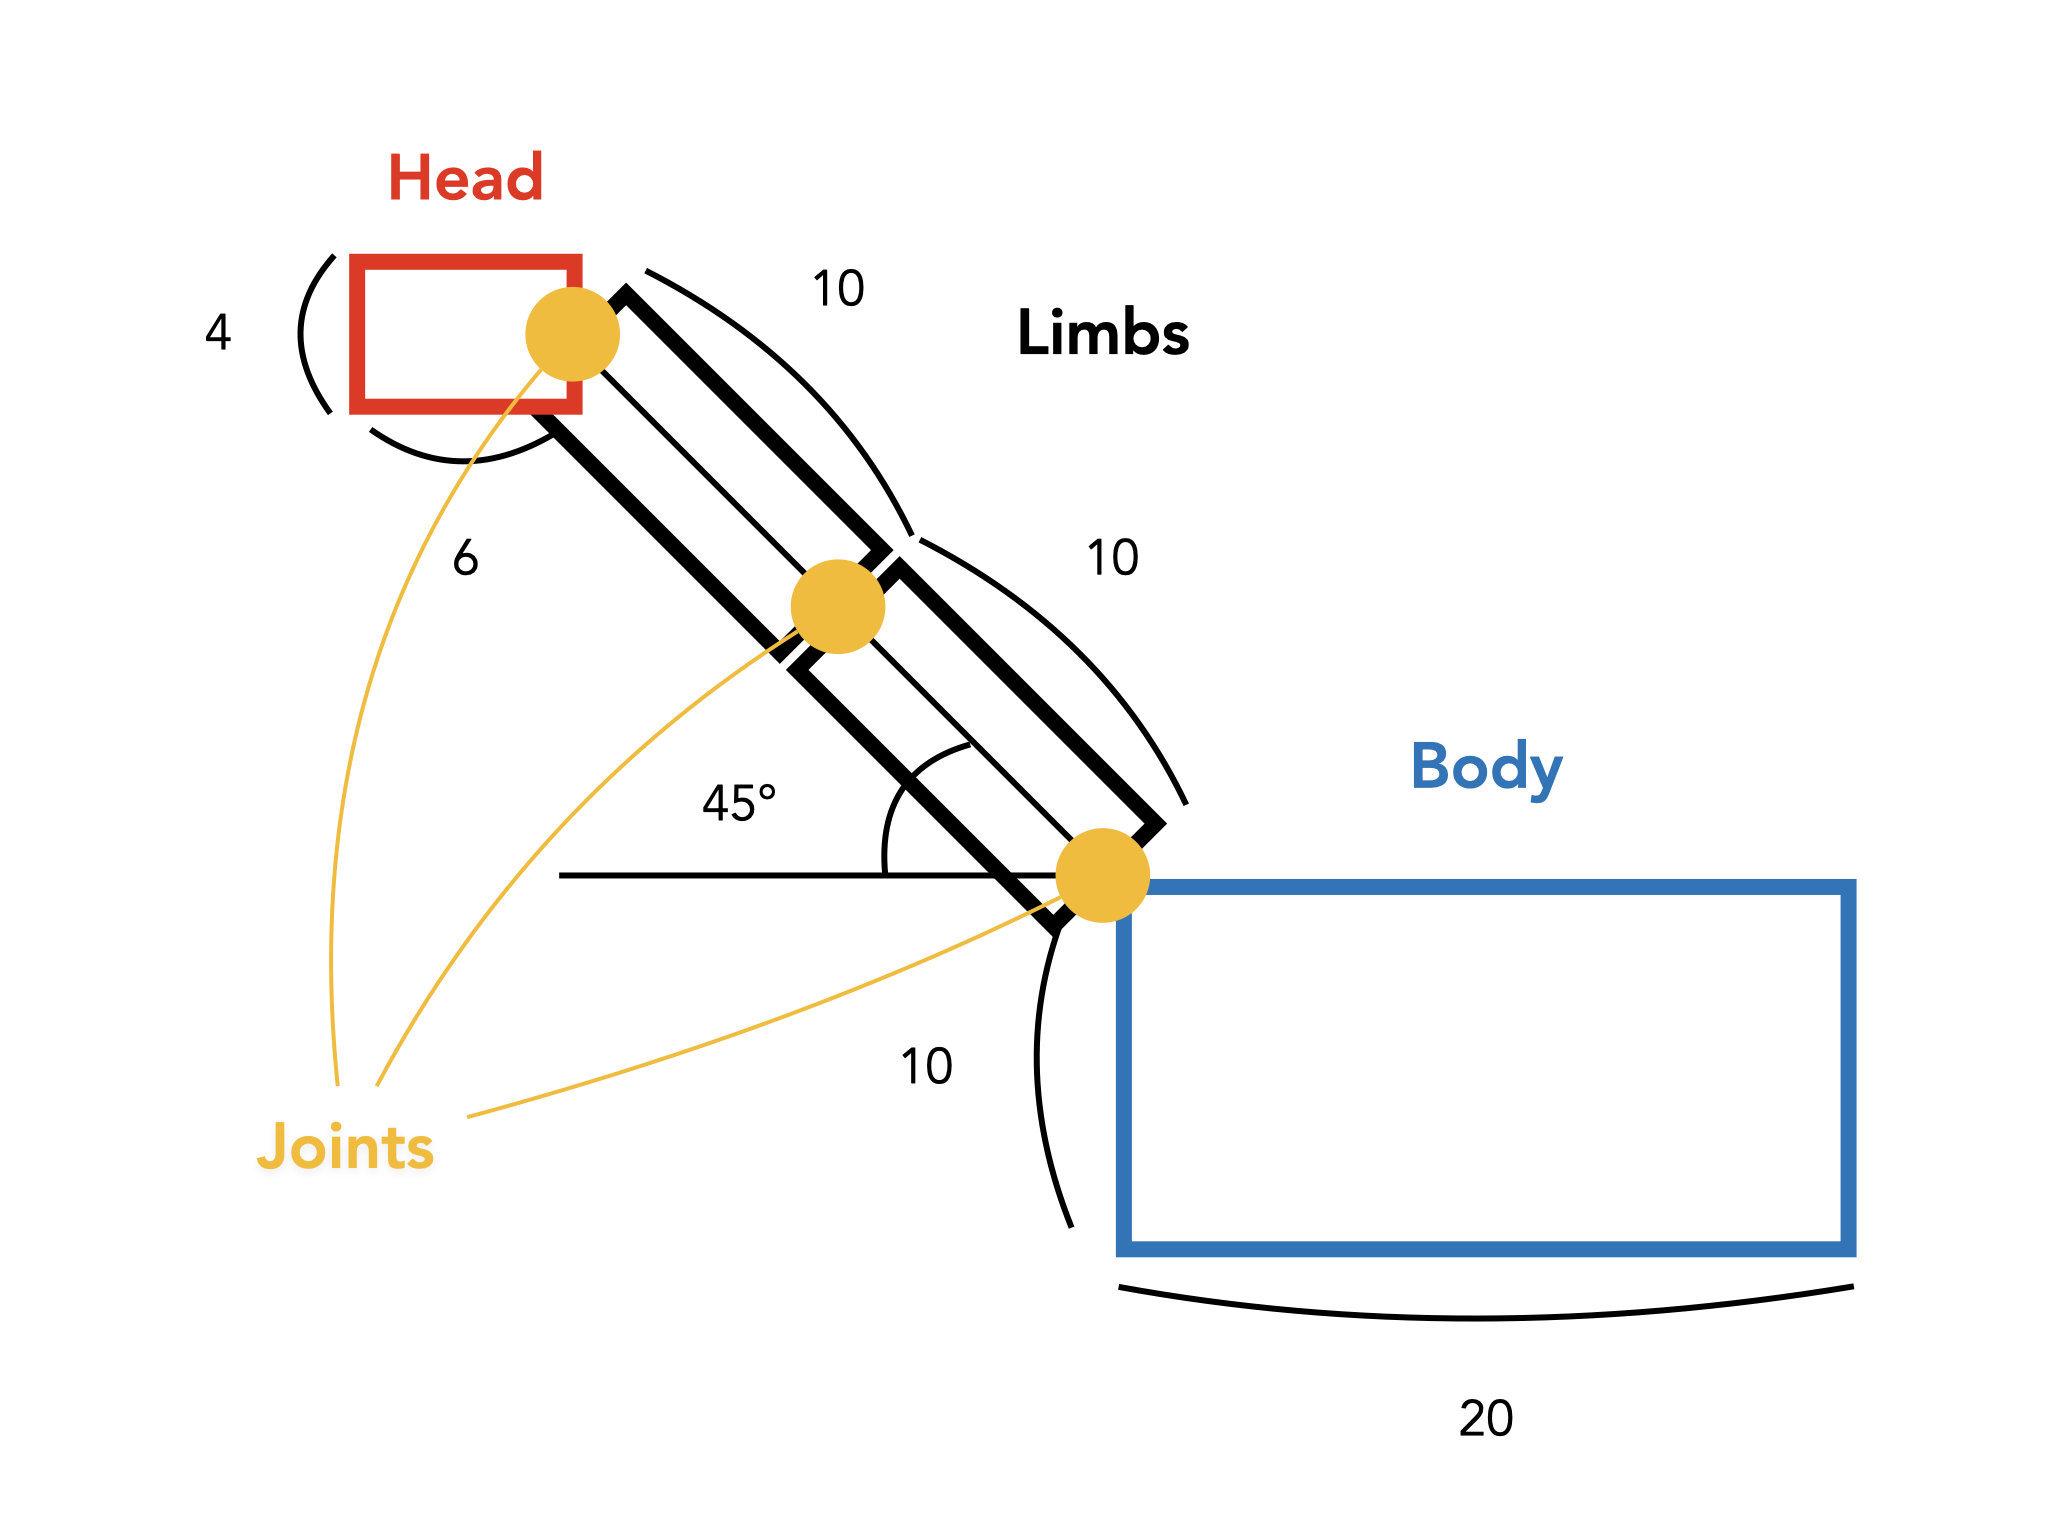
\includegraphics[width=1\textwidth]{figures/pigeon_diagram/pigeon_diagram_001.png}
        \caption{Diagram of the pigeon model}
        \label{fig:pigeon_dimension}
    \end{figure}
  Additionally, the pigeon's head relative to the body is facing the negative direction relative to the x-axis.
  The widths and heights of each limb, head, and body are $(10, 4)$, $(6, 4)$, $(20, 10)$ respectively.
  The initial angles of each limb are oriented at 45 degrees relative to the x-axis, and both the head and the body are oriented parallel to the x axis.
  The body's initial position is at the origin, and is set to move at a constant speed in the negative direction along the x-axis.

\section{Experiment Environments}
% details on all 5 params and reward function differences
  We trained a total of 5 reinforcement learning agents to control the pigeon model: 1 agent for the case where the model is given the baseline task given an unmoving body, 2 agents for cases where the model is given the same task with the body speed of 1, 2 agents for cases where the model is tasked to move its joints to maximize the reward function $r_{fifty\_fifty}$, as defined in Chapter \ref{ch:approach}, under the body speed of 0 and 1 respectively.

  % head target trajectory tracking
    Several additional variables are defined for the pigeon to execute the baseline task as shown in Figure \ref{fig:pigeon_target}.
      \begin{figure}[H]
          \centering
          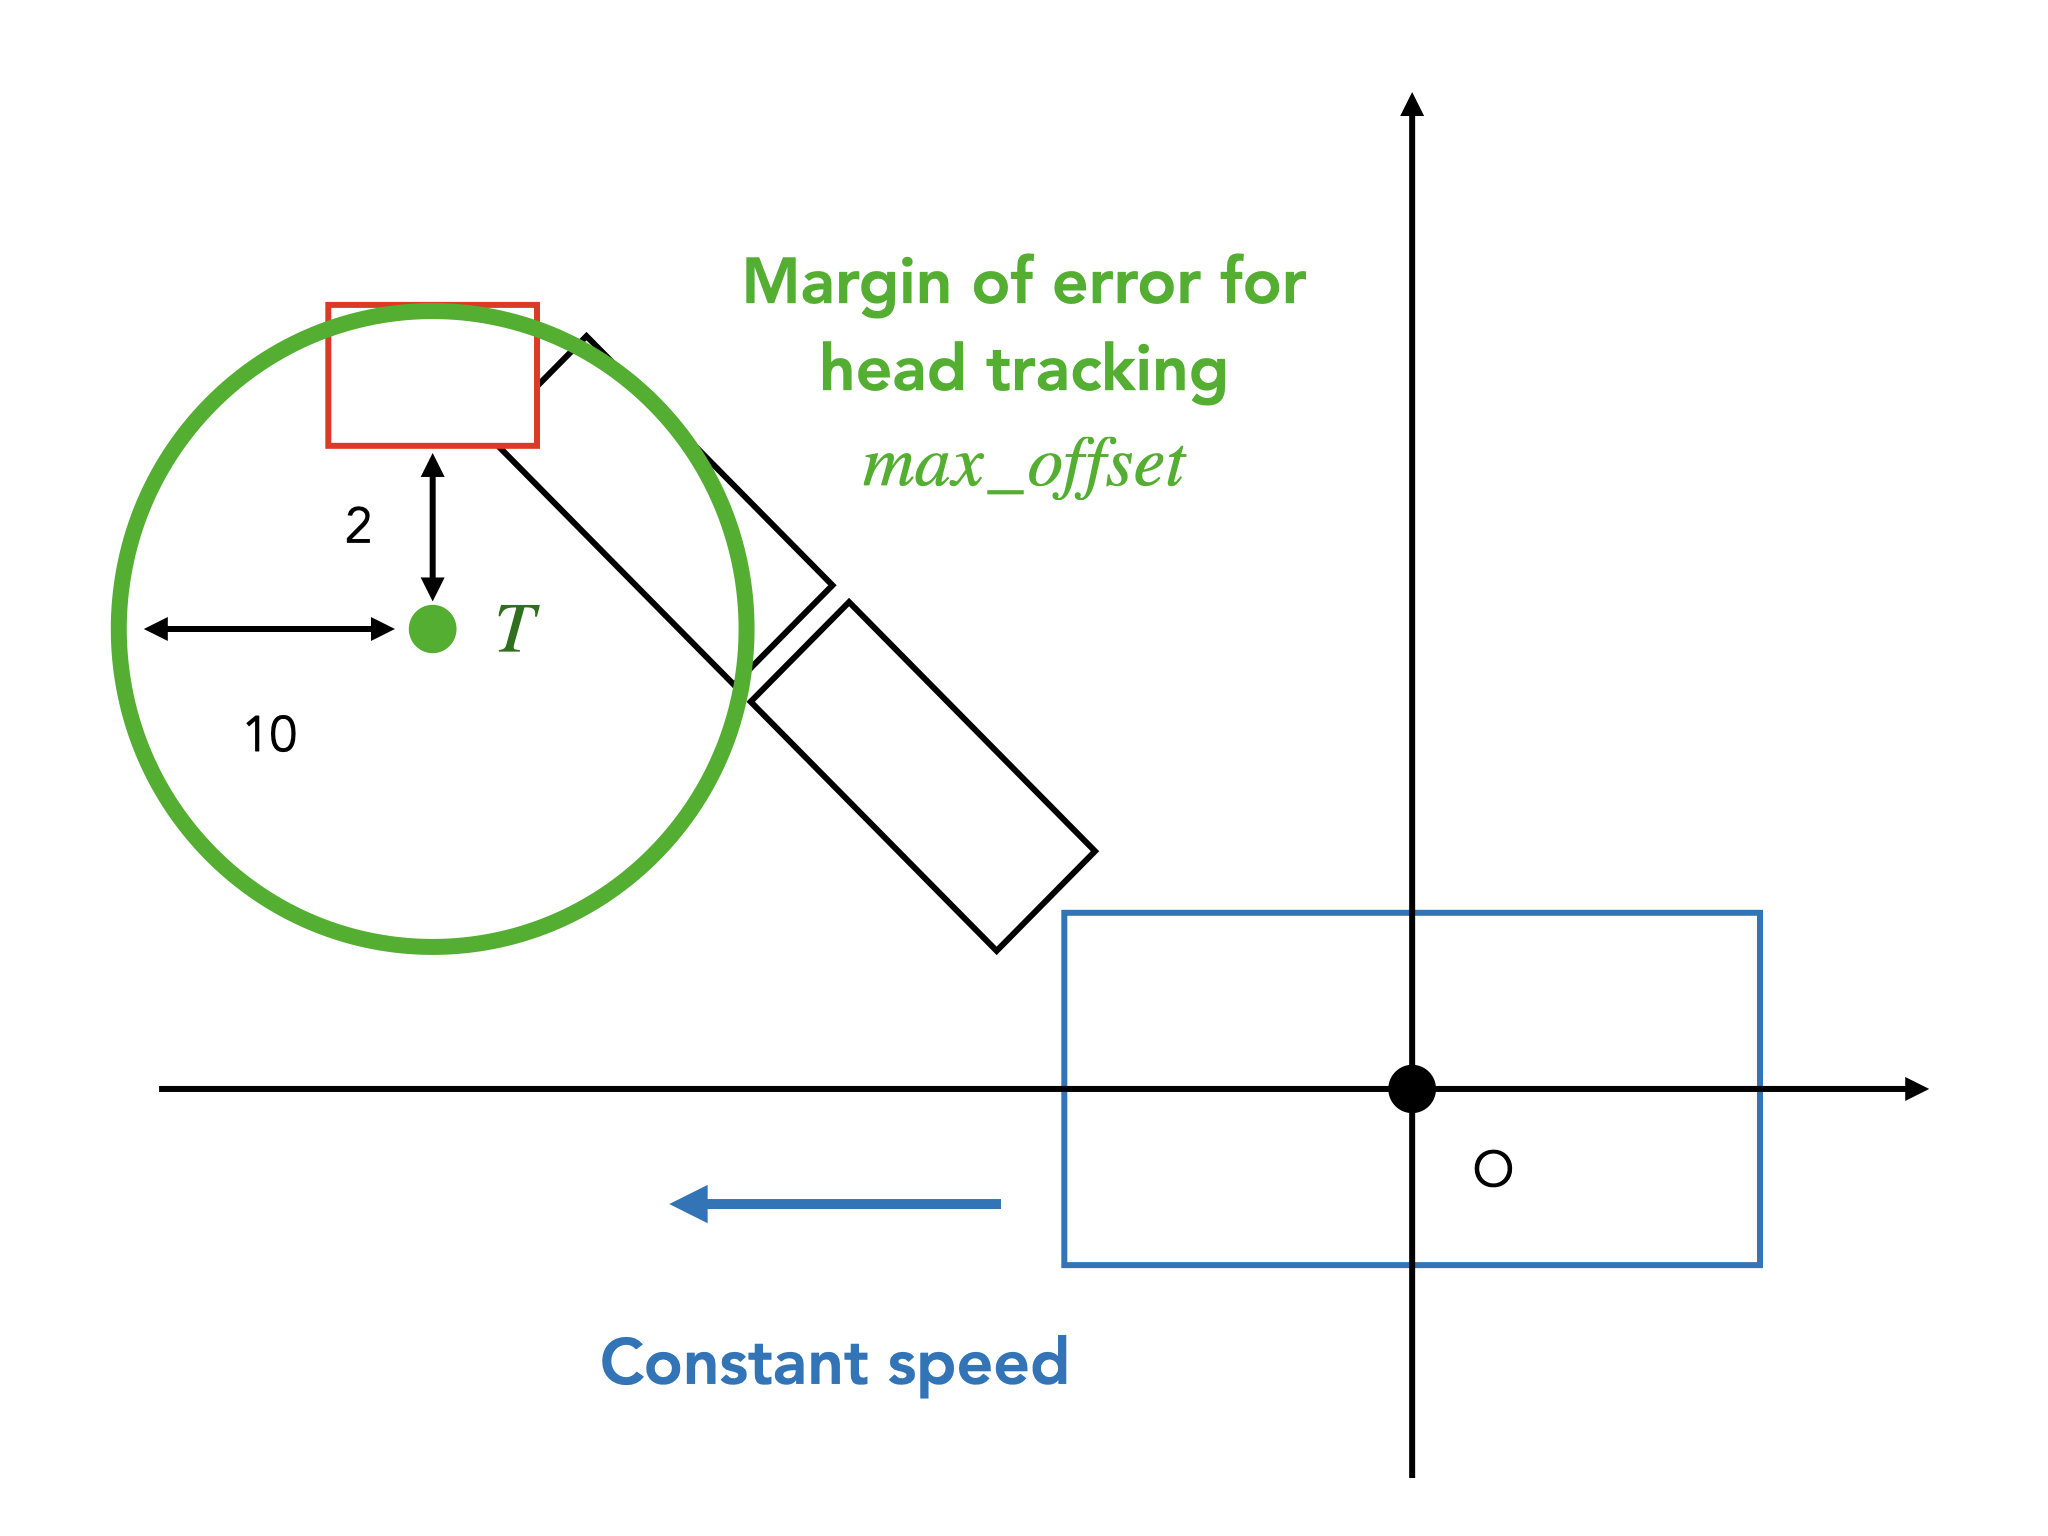
\includegraphics[width=1\textwidth]{figures/pigeon_diagram/pigeon_diagram_002.png}
          \label{fig:pigeon_target}
          \caption{Head trajectory tracking}
      \end{figure}
    $T$ is set at $(0, -2)$ relative to the initial position of the head.
    We set the threshold value for the distance between the target position and the torso's position to 10. As mentioned in Chapter \ref{ch:approach} when the the said distance is below the threshold value, $T$ is reset to be the same position relative to the body as its initial position.
    We set a value $max\_offset$ that represents the margin of error between $T$ and the position of the head.

    % speed = 0
      % _head_stable_manual_reposition_strict_angle
        For the case with an unmoving body, we define a function that generates positive rewards only for timesteps where the distance between the head and $T$ is within $max\_offset = 0.5$. Each reward is bounded within $[0, 1]$ and scaled based on the level of alignment to the x-axis.
          \begin{equation}
              {r_{head\_stable\_manual\_reposition\_strict\_angle}}_t =
              \begin{cases}
                  1 - \frac {\alpha_t} \pi & \text{if $\alpha_t < \frac \pi 6$} \\
                  0 & \text{otherwise}
              \end{cases}
          \end{equation}
        where $\alpha_t$ is the angle of the head at timestep $t$.

    % speed = 1
      % _head_stable_manual_reposition
        For the speed of 1, unlike the case with the unmoving body, $max\_offset = 1$.
        Additionally, alongside $r_{head\_stable\_manual\_reposition\_strict\_angle}$, we define a looser reward function that generates positive rewards as long as the head is within the set margin of error around the target location.
        It is expected that this function would serve as an alternate less strict to the former reward function that produce similar behaviors.
        \begin{equation}
          \begin{aligned}
            {r_{head\_stable\_manual\_reposition}}_t = {r_{head\_stable\_manual\_reposition\_strict\_angle}}_t + \\
              \begin{cases}
                  1 - \frac {\delta_t} {max\_offset} & \text{$\delta_t < max\_offset$} \\
                  0 & \text{otherwise}
              \end{cases}
          \end{aligned}
        \end{equation}
        where $\delta_t$ is the distance between the head and $T$ at timestep $t$.

  % _fifty_fifty
    Preliminary hypotheses regarding retinal stabilization and motion parallax are depicted as the reward function $r_{fifty\_fifty}$. The reward function is used to train agents that represent behaviors derived from such hypotheses under the conditions of both speeds 0 and 1. For both cases, $max\_offset = 1$.
    % external objects
      3 points and their positions are defined to represent 1 static and 2 dynamic objects placed on the surrounding environment of the pigeon.
      The static object's position is $(-30.0, 30.0)$, and the 2 dynamic objects' positions are $(-30.0, 60.0)$, $(-60.0, 30.0)$. The former dynamic object moves at speed 1 in the positive direction along the x-axis, while the latter moves at the same speed in the negative direction along the x-axis.

We constructed OpenAI Gym \cite{brockman2016openai} environments \lstinline|PigeonEnv3Joints| and \lstinline|PigeonRetinalEnv| for conducting reinforcement learning based on the baseline and preliminary hypotheses, respectively.
  Details regarding the environments' code are in Appendix \ref{append:1}.

\section{Reinforcement Learning}
We used SAC to conduct batch training on each deep neural network agent for 3000 epochs. Each deep neural network has one hidden layer containing 256 neurons. Details regarding more rigorous hyperparameter settings are in Appendix \ref{append:2}.

% why we didn't use PPO
  PPO, despite being used often as baseline for many reinforcement learning experiments as we have stated beforehand, was not used for training any of the 5 aforementioned controllers.
  When we attempted to train deep neural network controllers for pigeon models with static bodies using PPO and SAC with $r_{head\_stable\_manual\_reposition}$, we found that the agent trained on SAC had a more stable learning curve and a faster convergence rate than the agent trained on PPO.
  Therefore, we determined that it would be more reliable to use SAC to obtain the desired results.

  \chapter{Results}

% pre-figure explanation
  We rendered the resulting behaviors produced by controllers trained on aforementioned reward functions and environments into images or frames.
  Combining the frames generated for each of the 1000 timesteps and setting as 60 frames per second resulted in 33.35 second videos.
  The time-lapses presented in Figures \ref{fig:manual_trajectory_body_speed_0}, \ref{fig:manual_trajectory_strict_body_speed_1}, \ref{fig:manual_trajectory_not_strict_body_speed_1}, \ref{fig:fifty_fifty_body_speed_0}, and \ref{fig:fifty_fifty_body_speed_1} were created by sampling every $300$ frames within the last 30 seconds of the video.
  The frames' sequential order is from the top left to the bottom right.
  The camera is locked to follow the pigeon's body.
  % 60/5 * [10] = 300


  \begin{figure}[H]
      \centering
      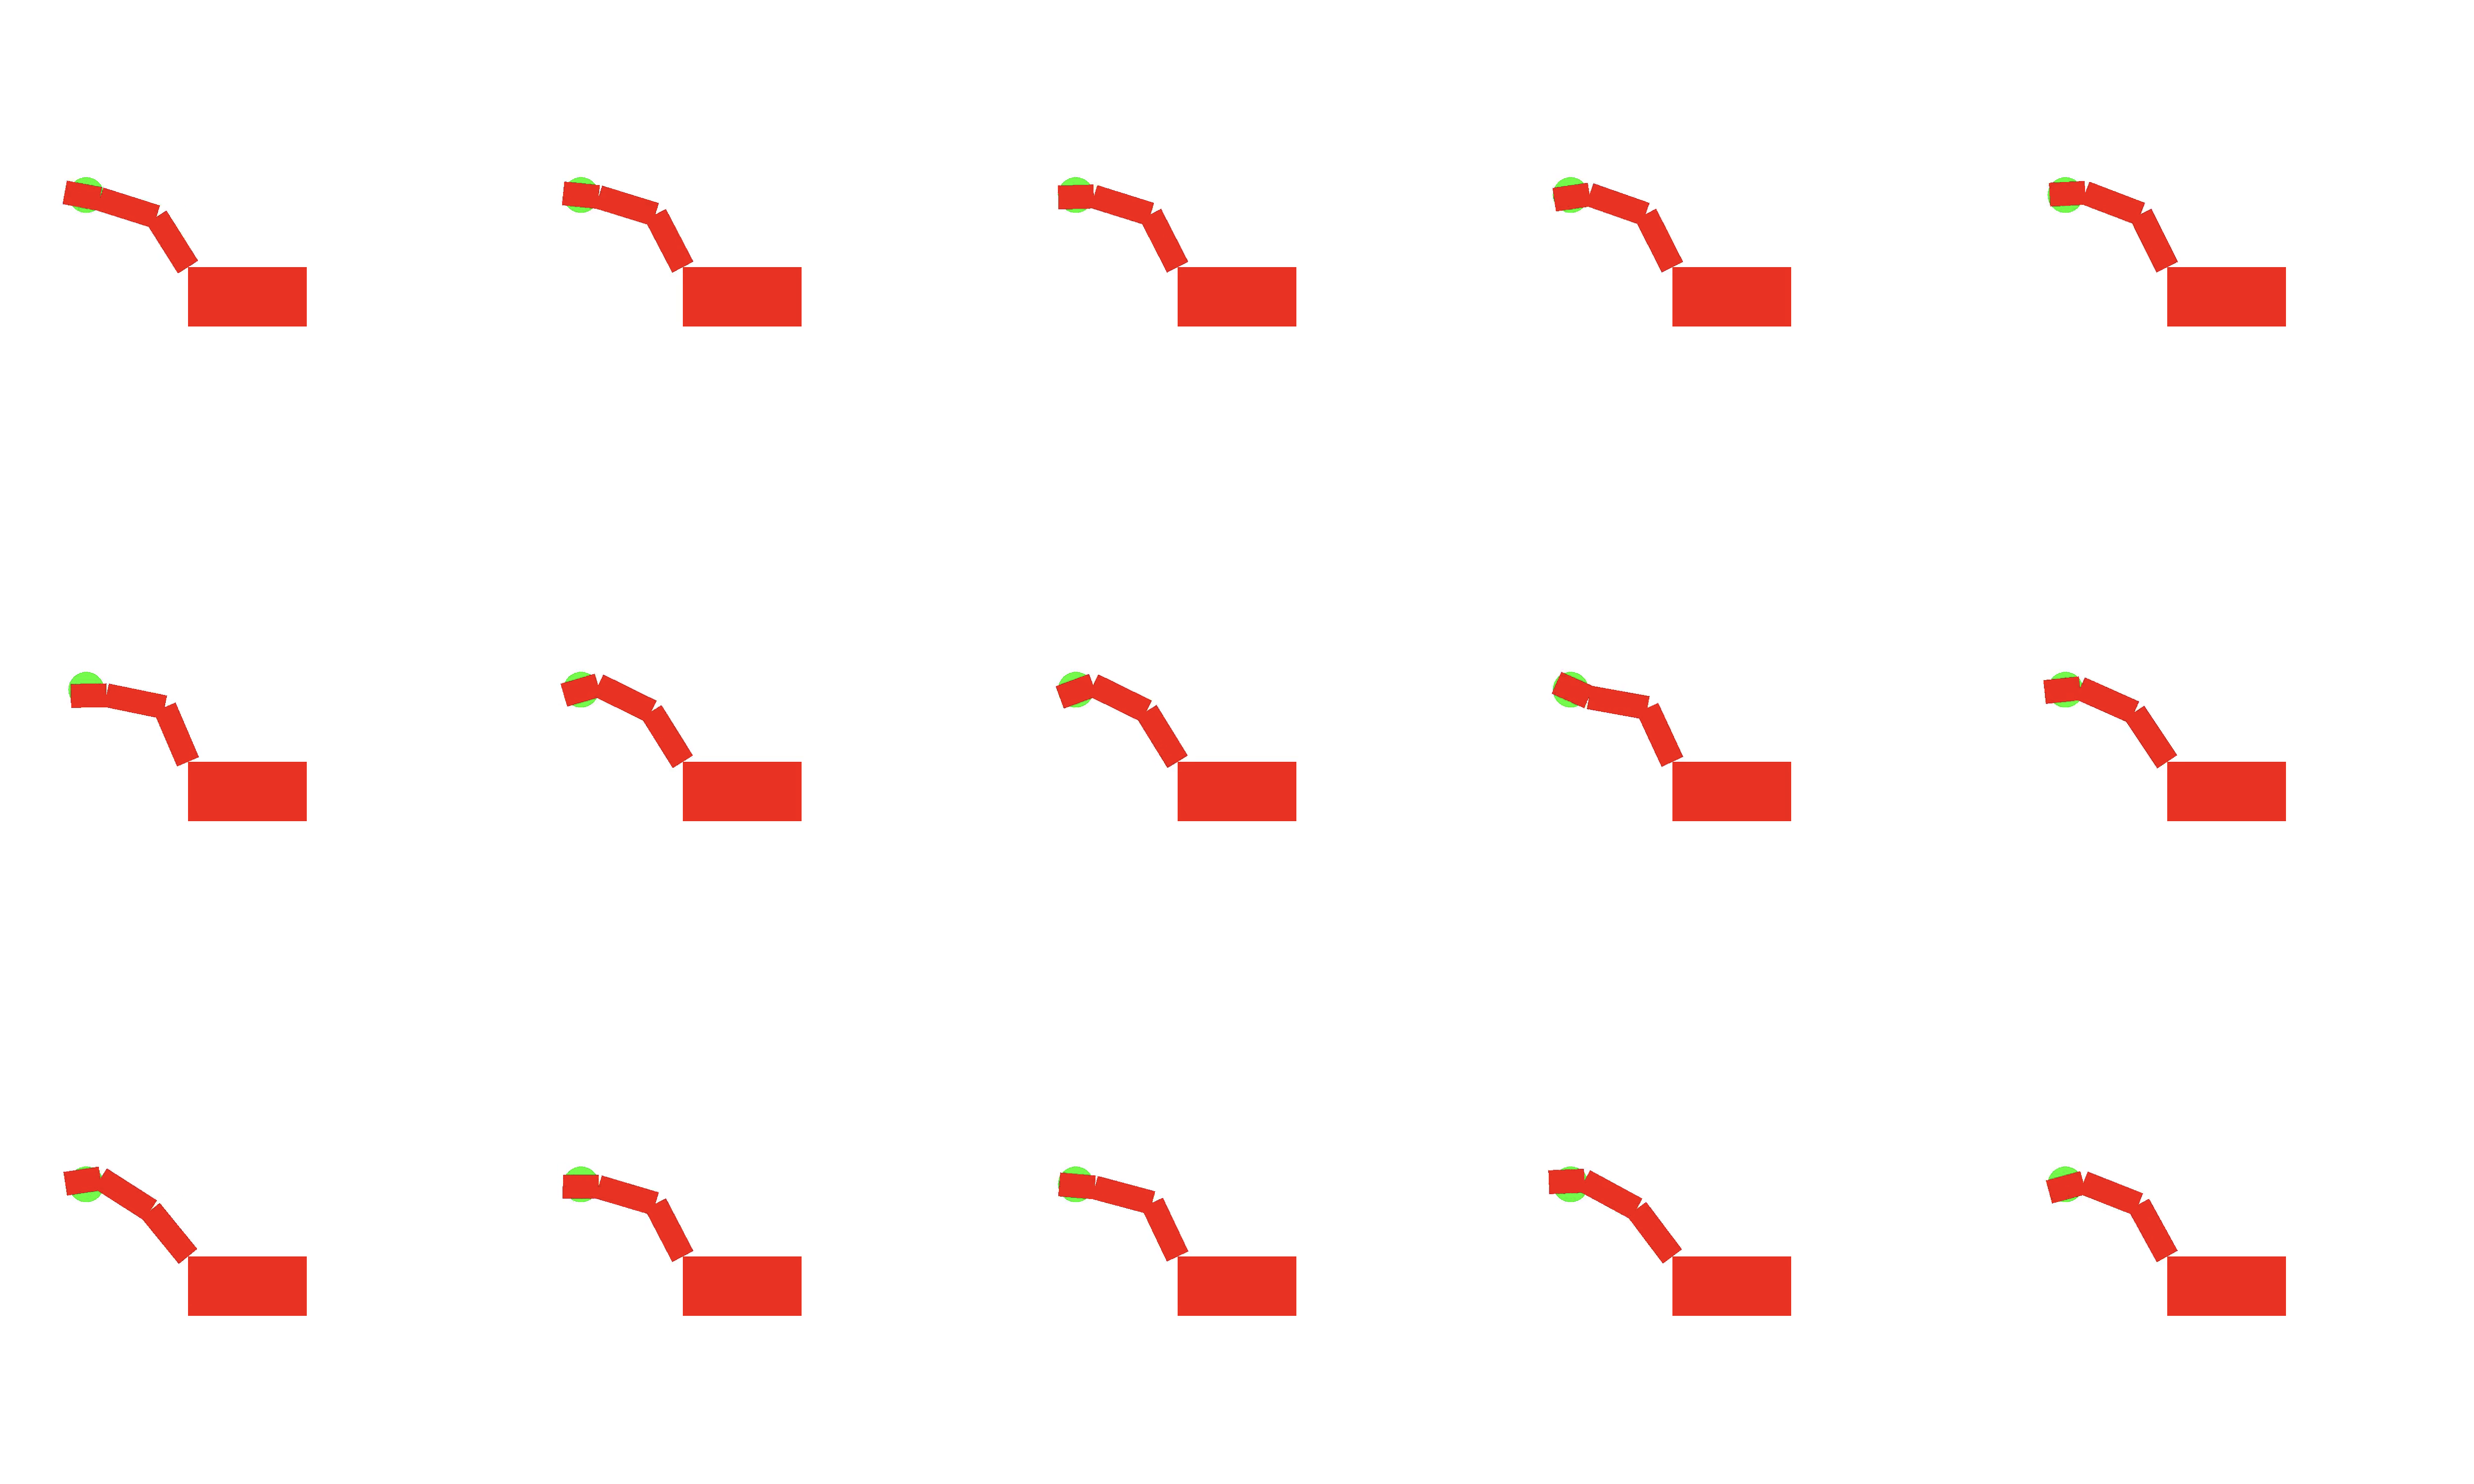
\includegraphics[width=1\textwidth]{figures/frames/frames_001.png}
      \caption{Control of a pigeon model with a static body trained on $r_{head\_stable\_manual\_reposition\_strict\_angle}$ with $max\_offset = 0.5$. The green circle indicate the margin of error around the target head location defined by $max\_offset$.}
      \label{fig:manual_trajectory_body_speed_0}
  \end{figure}

  \begin{figure}[H]
      \centering
      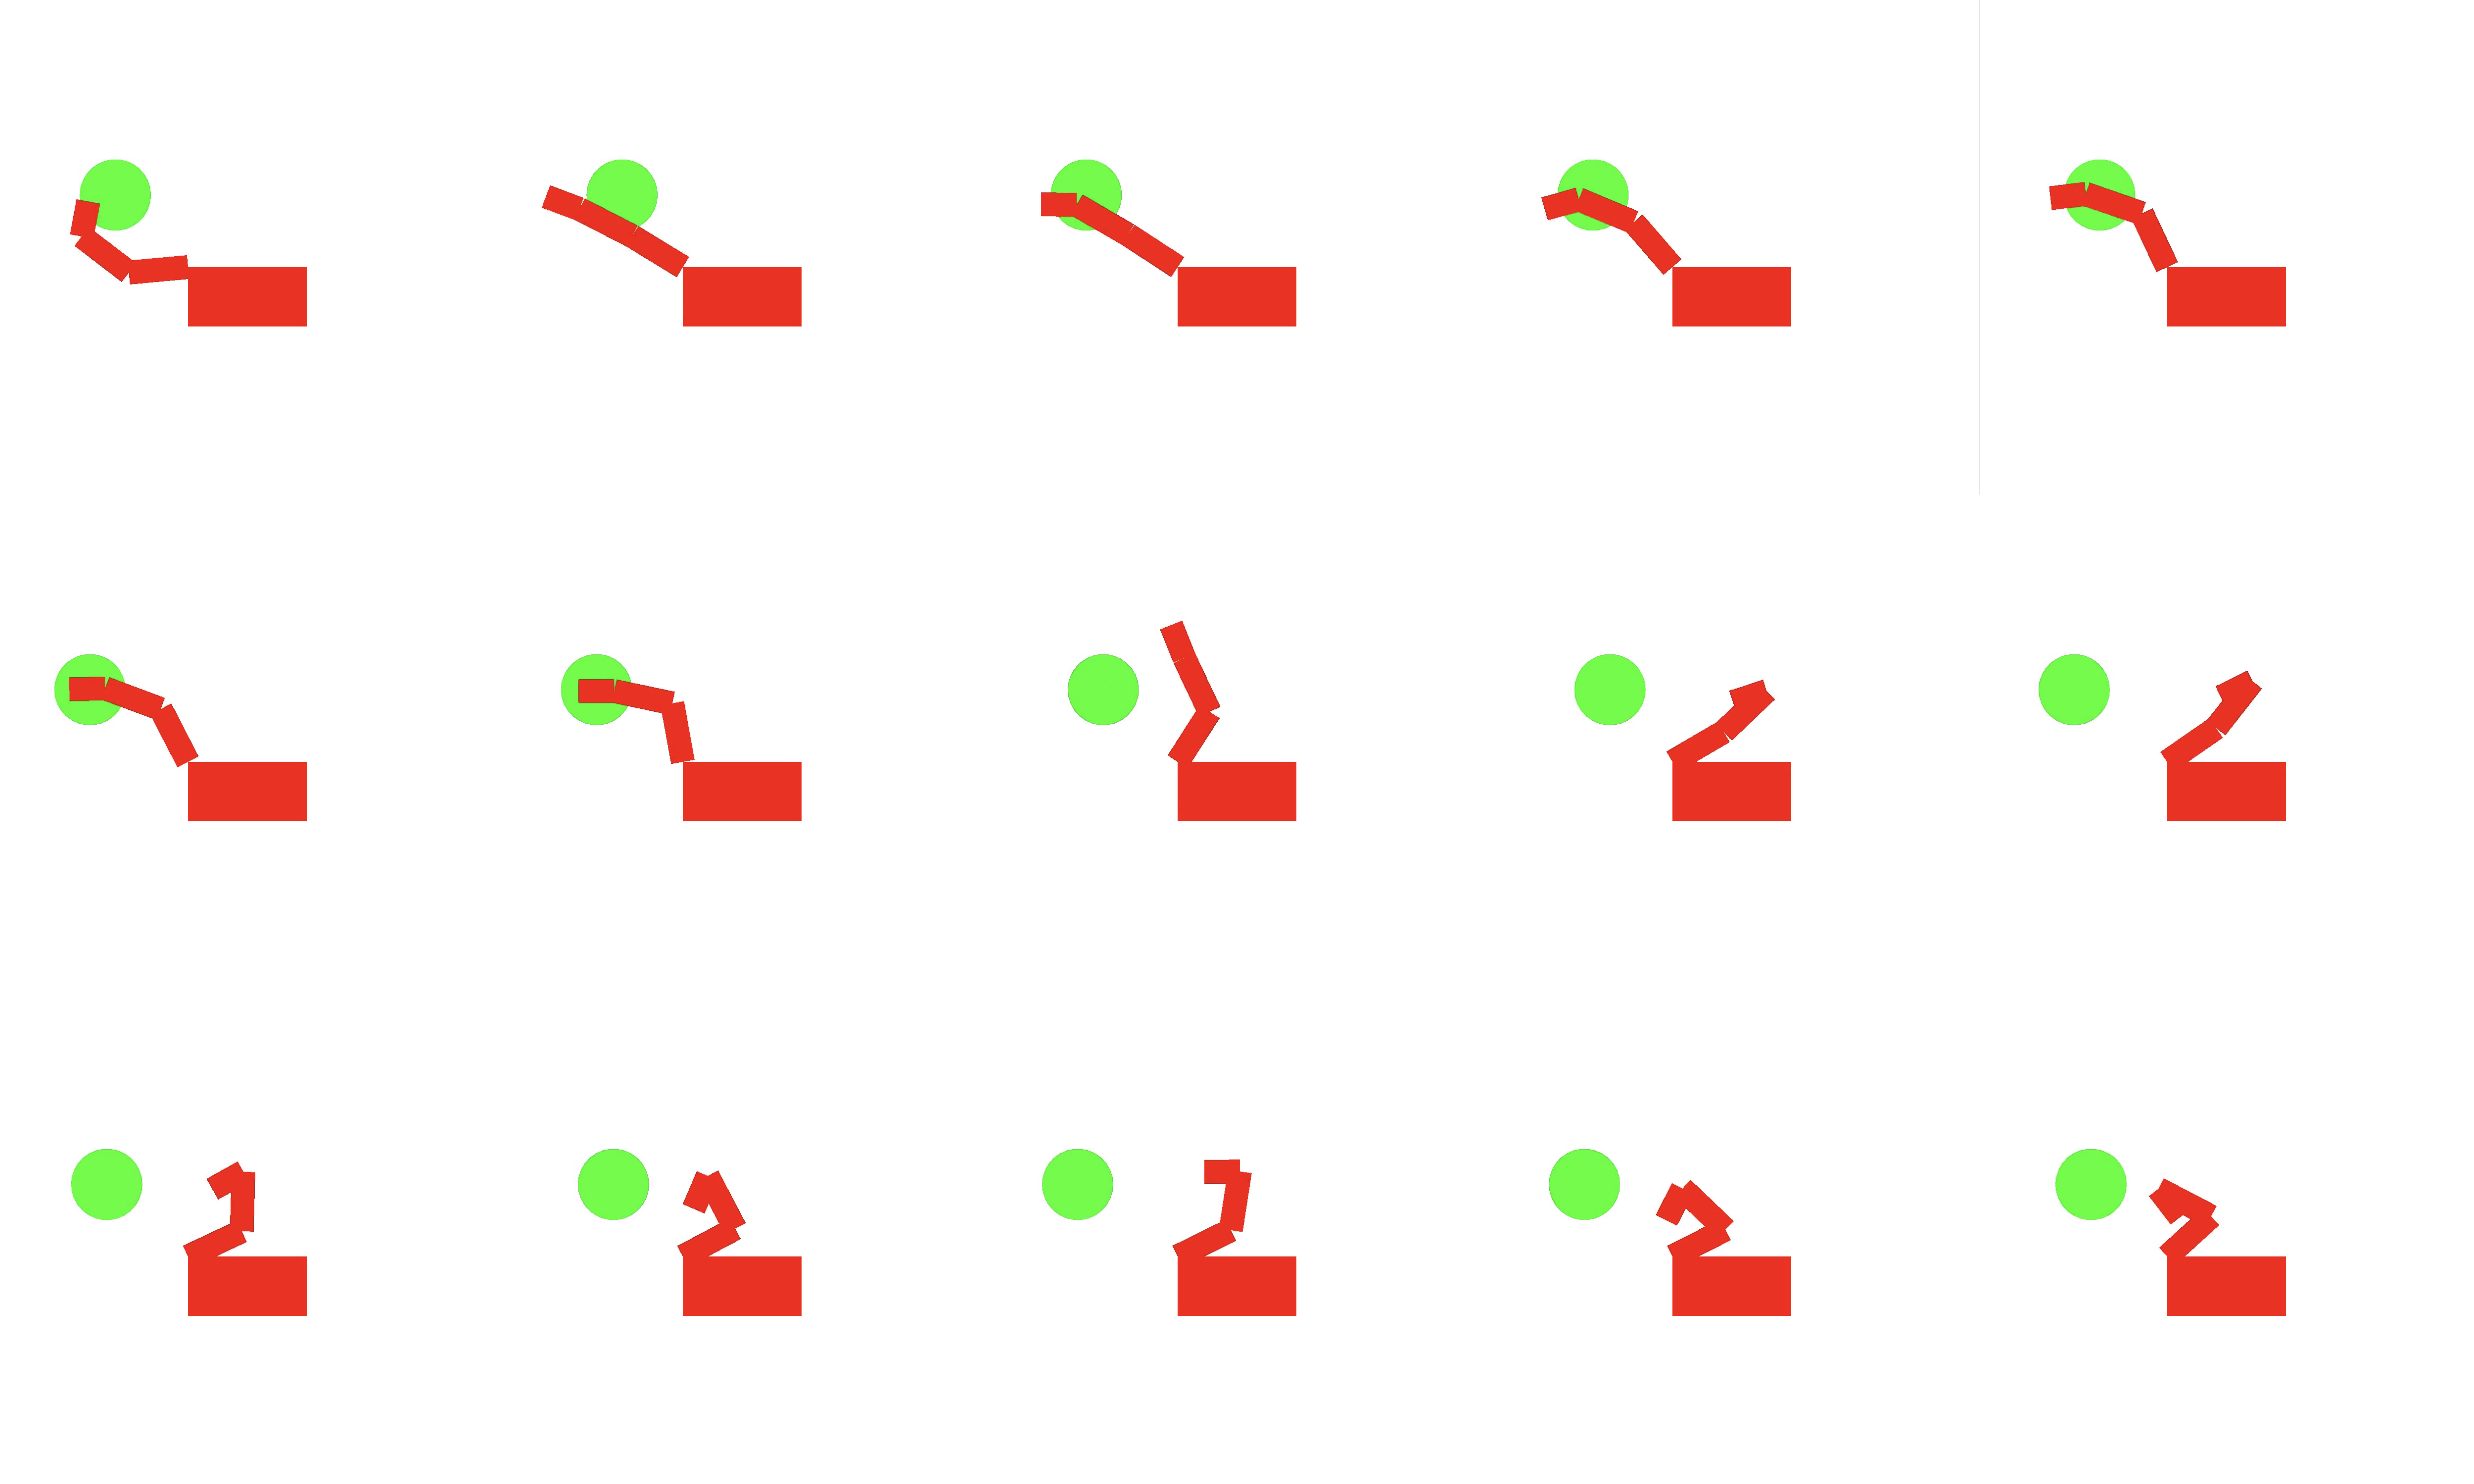
\includegraphics[width=1\textwidth]{figures/frames/frames_002.png}
      \caption{Control of a pigeon model with the body speed of 1 trained on $r_{head\_stable\_manual\_reposition\_strict\_angle}$ with $max\_offset = 1.0$. The green circle indicate the margin of error around the target head location defined by $max\_offset$.}
      \label{fig:manual_trajectory_strict_body_speed_1}
  \end{figure}

  \begin{figure}[H]
      \centering
      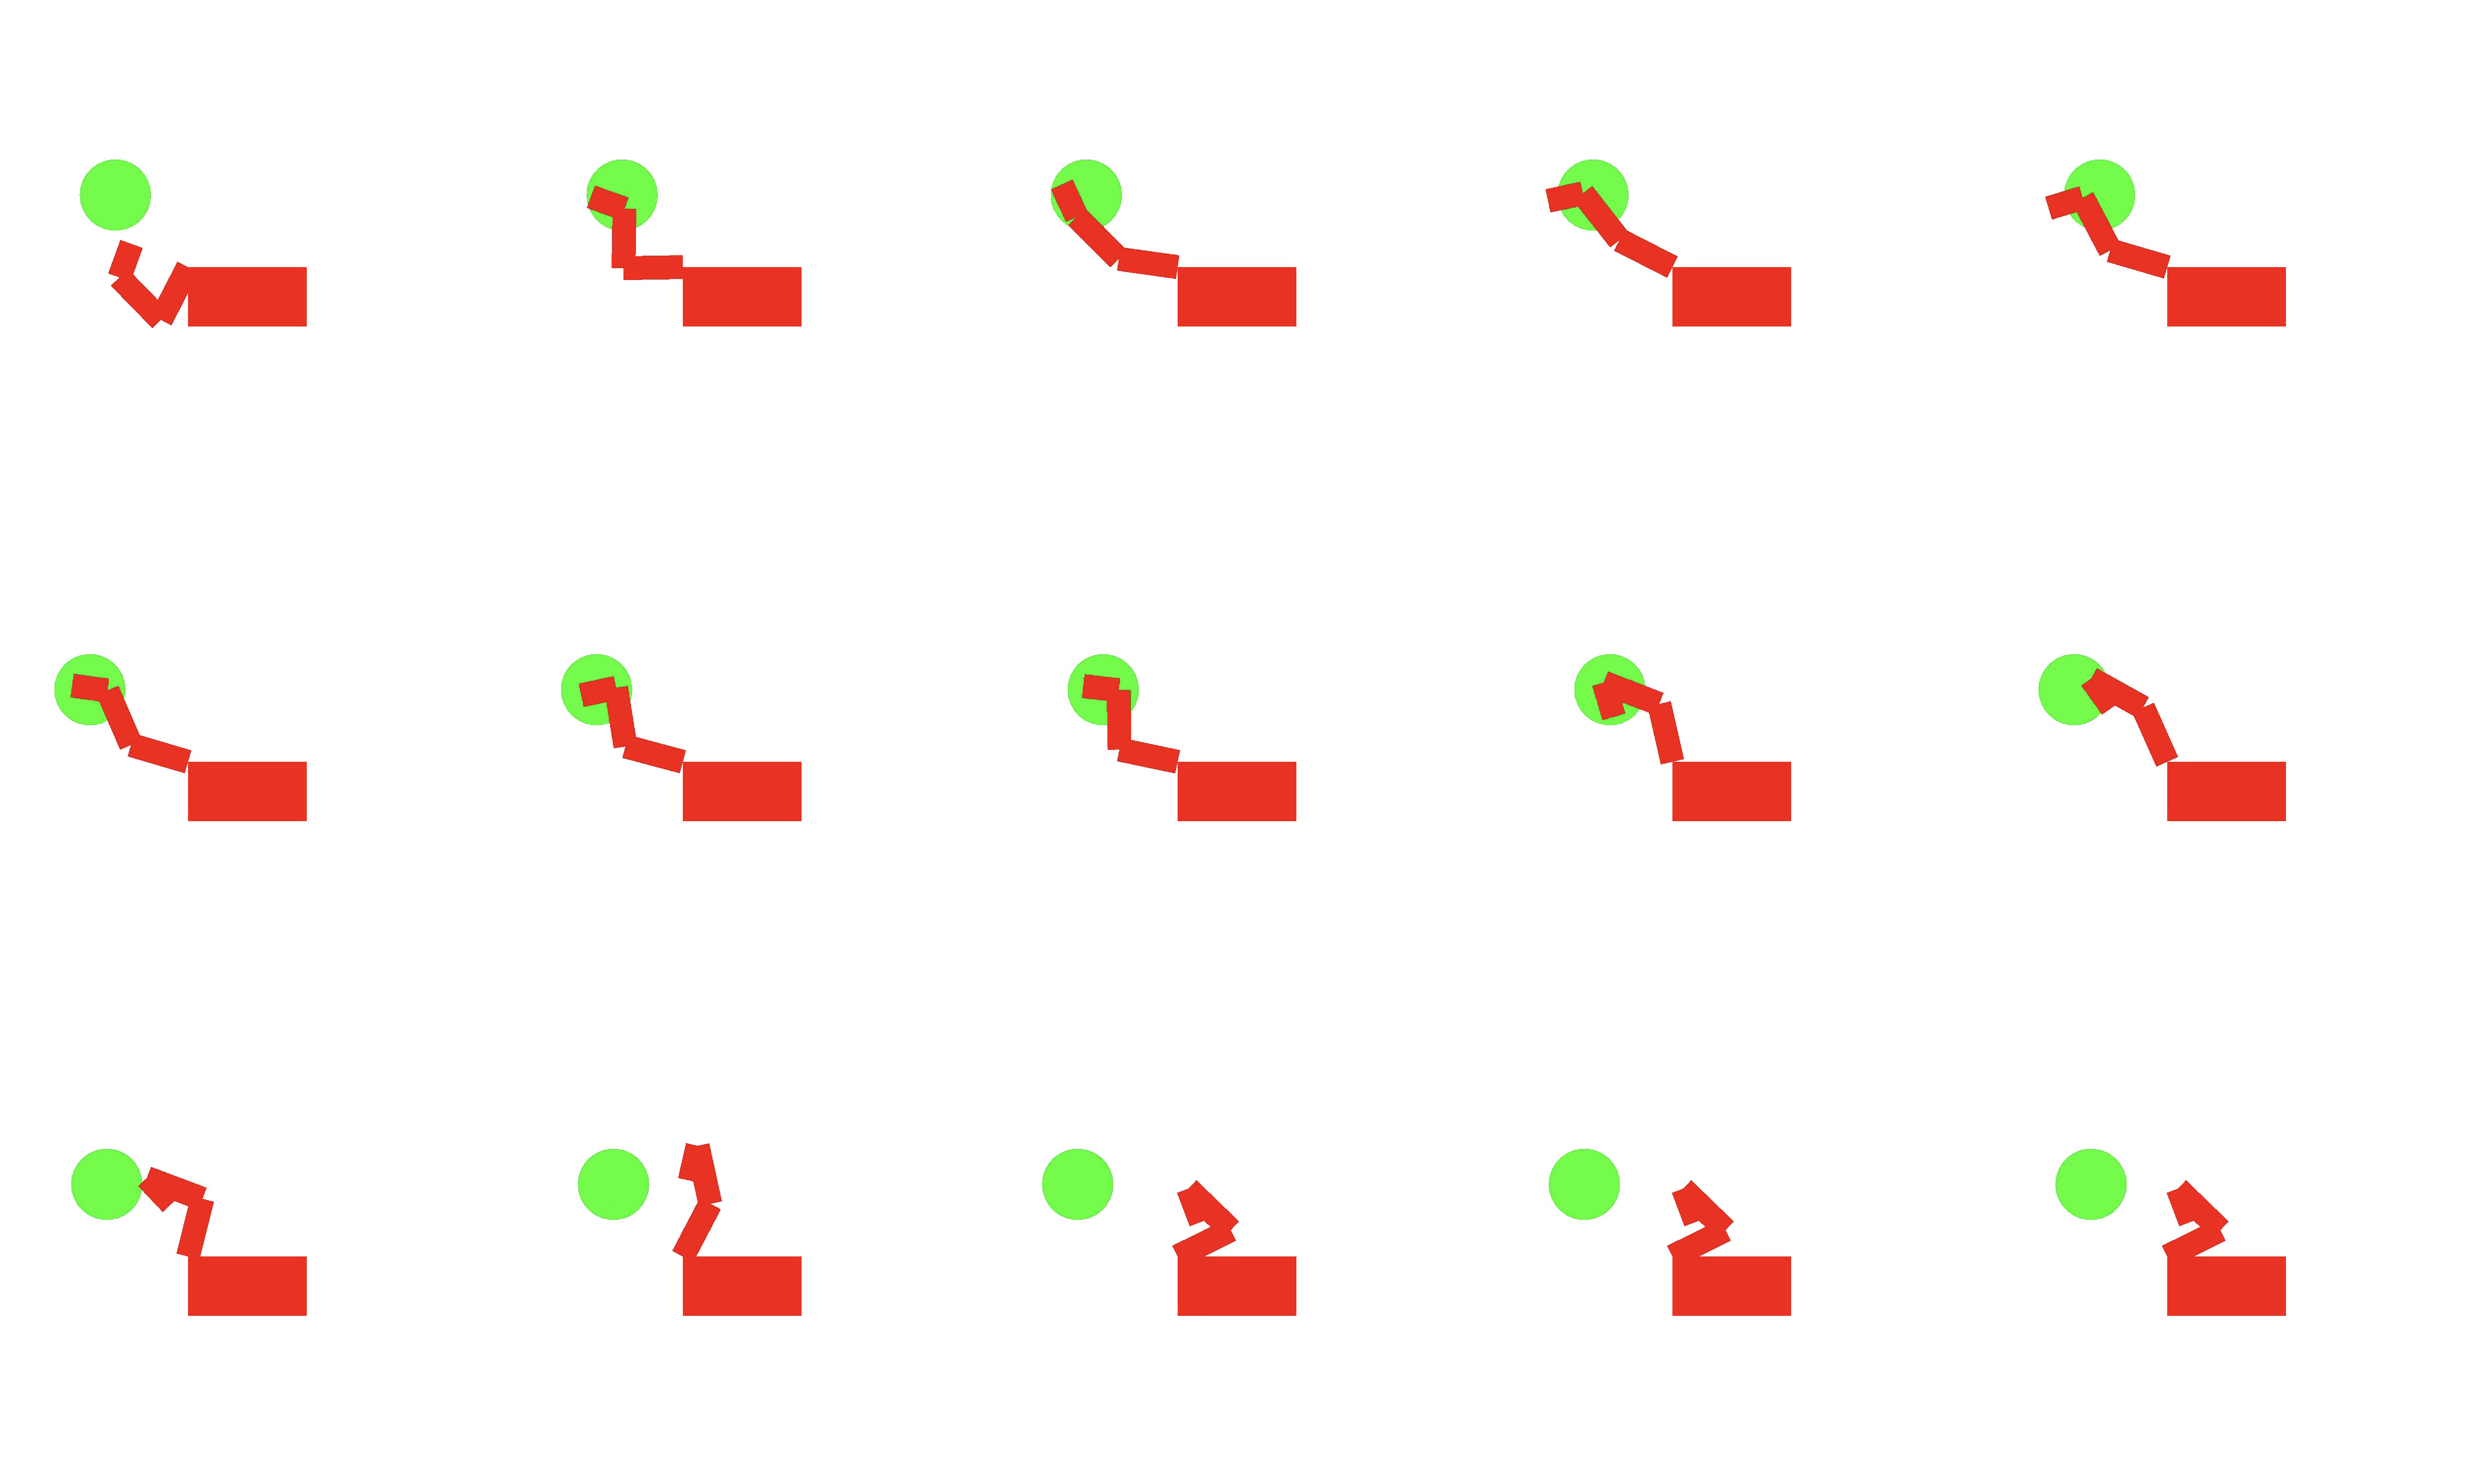
\includegraphics[width=1\textwidth]{figures/frames/frames_003.png}
      \caption{Control of a pigeon model with the body speed of 1 trained on $r_{head\_stable\_manual\_reposition}$ with $max\_offset = 1.0$. The green circle indicate the margin of error around the target head location defined by $max\_offset$.}
      \label{fig:manual_trajectory_not_strict_body_speed_1}
  \end{figure}

  \begin{figure}[H]
      \centering
      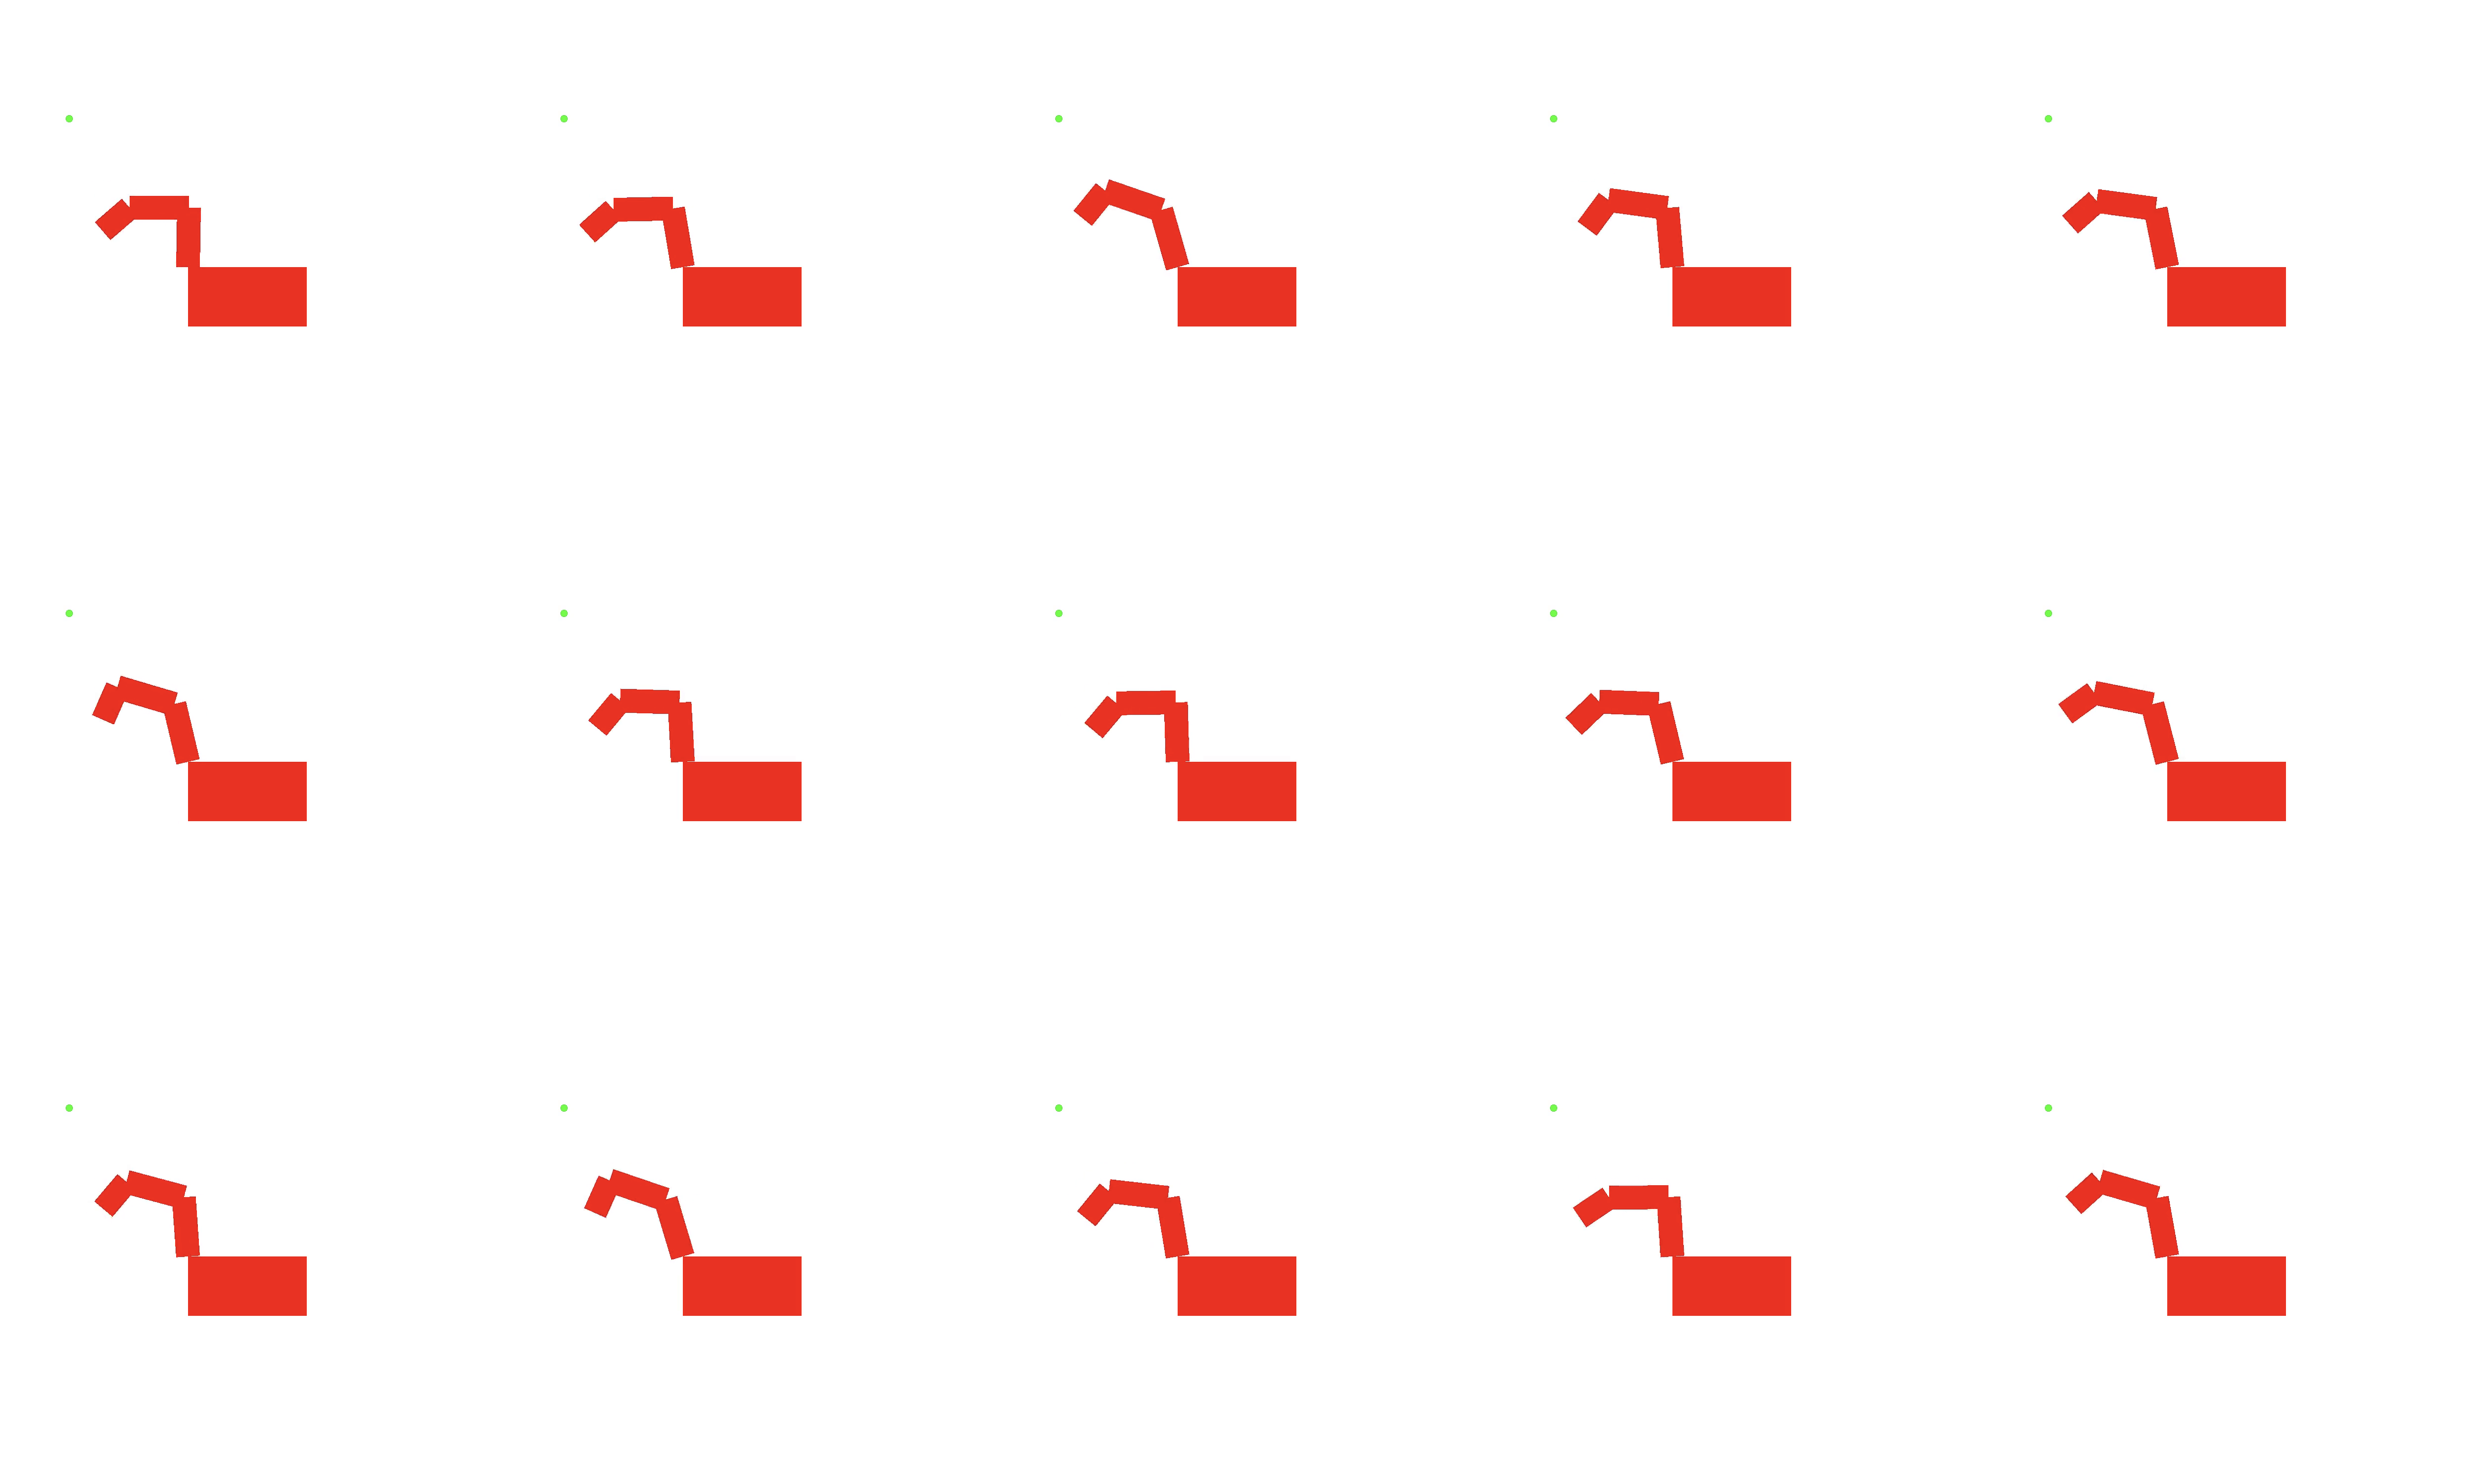
\includegraphics[width=1\textwidth]{figures/frames/frames_004.png}
      \caption{Control of a pigeon model with a static body trained on $r_{fifty\_fifty}$}
      \label{fig:fifty_fifty_body_speed_0}
  \end{figure}

  \begin{figure}[H]
      \centering
      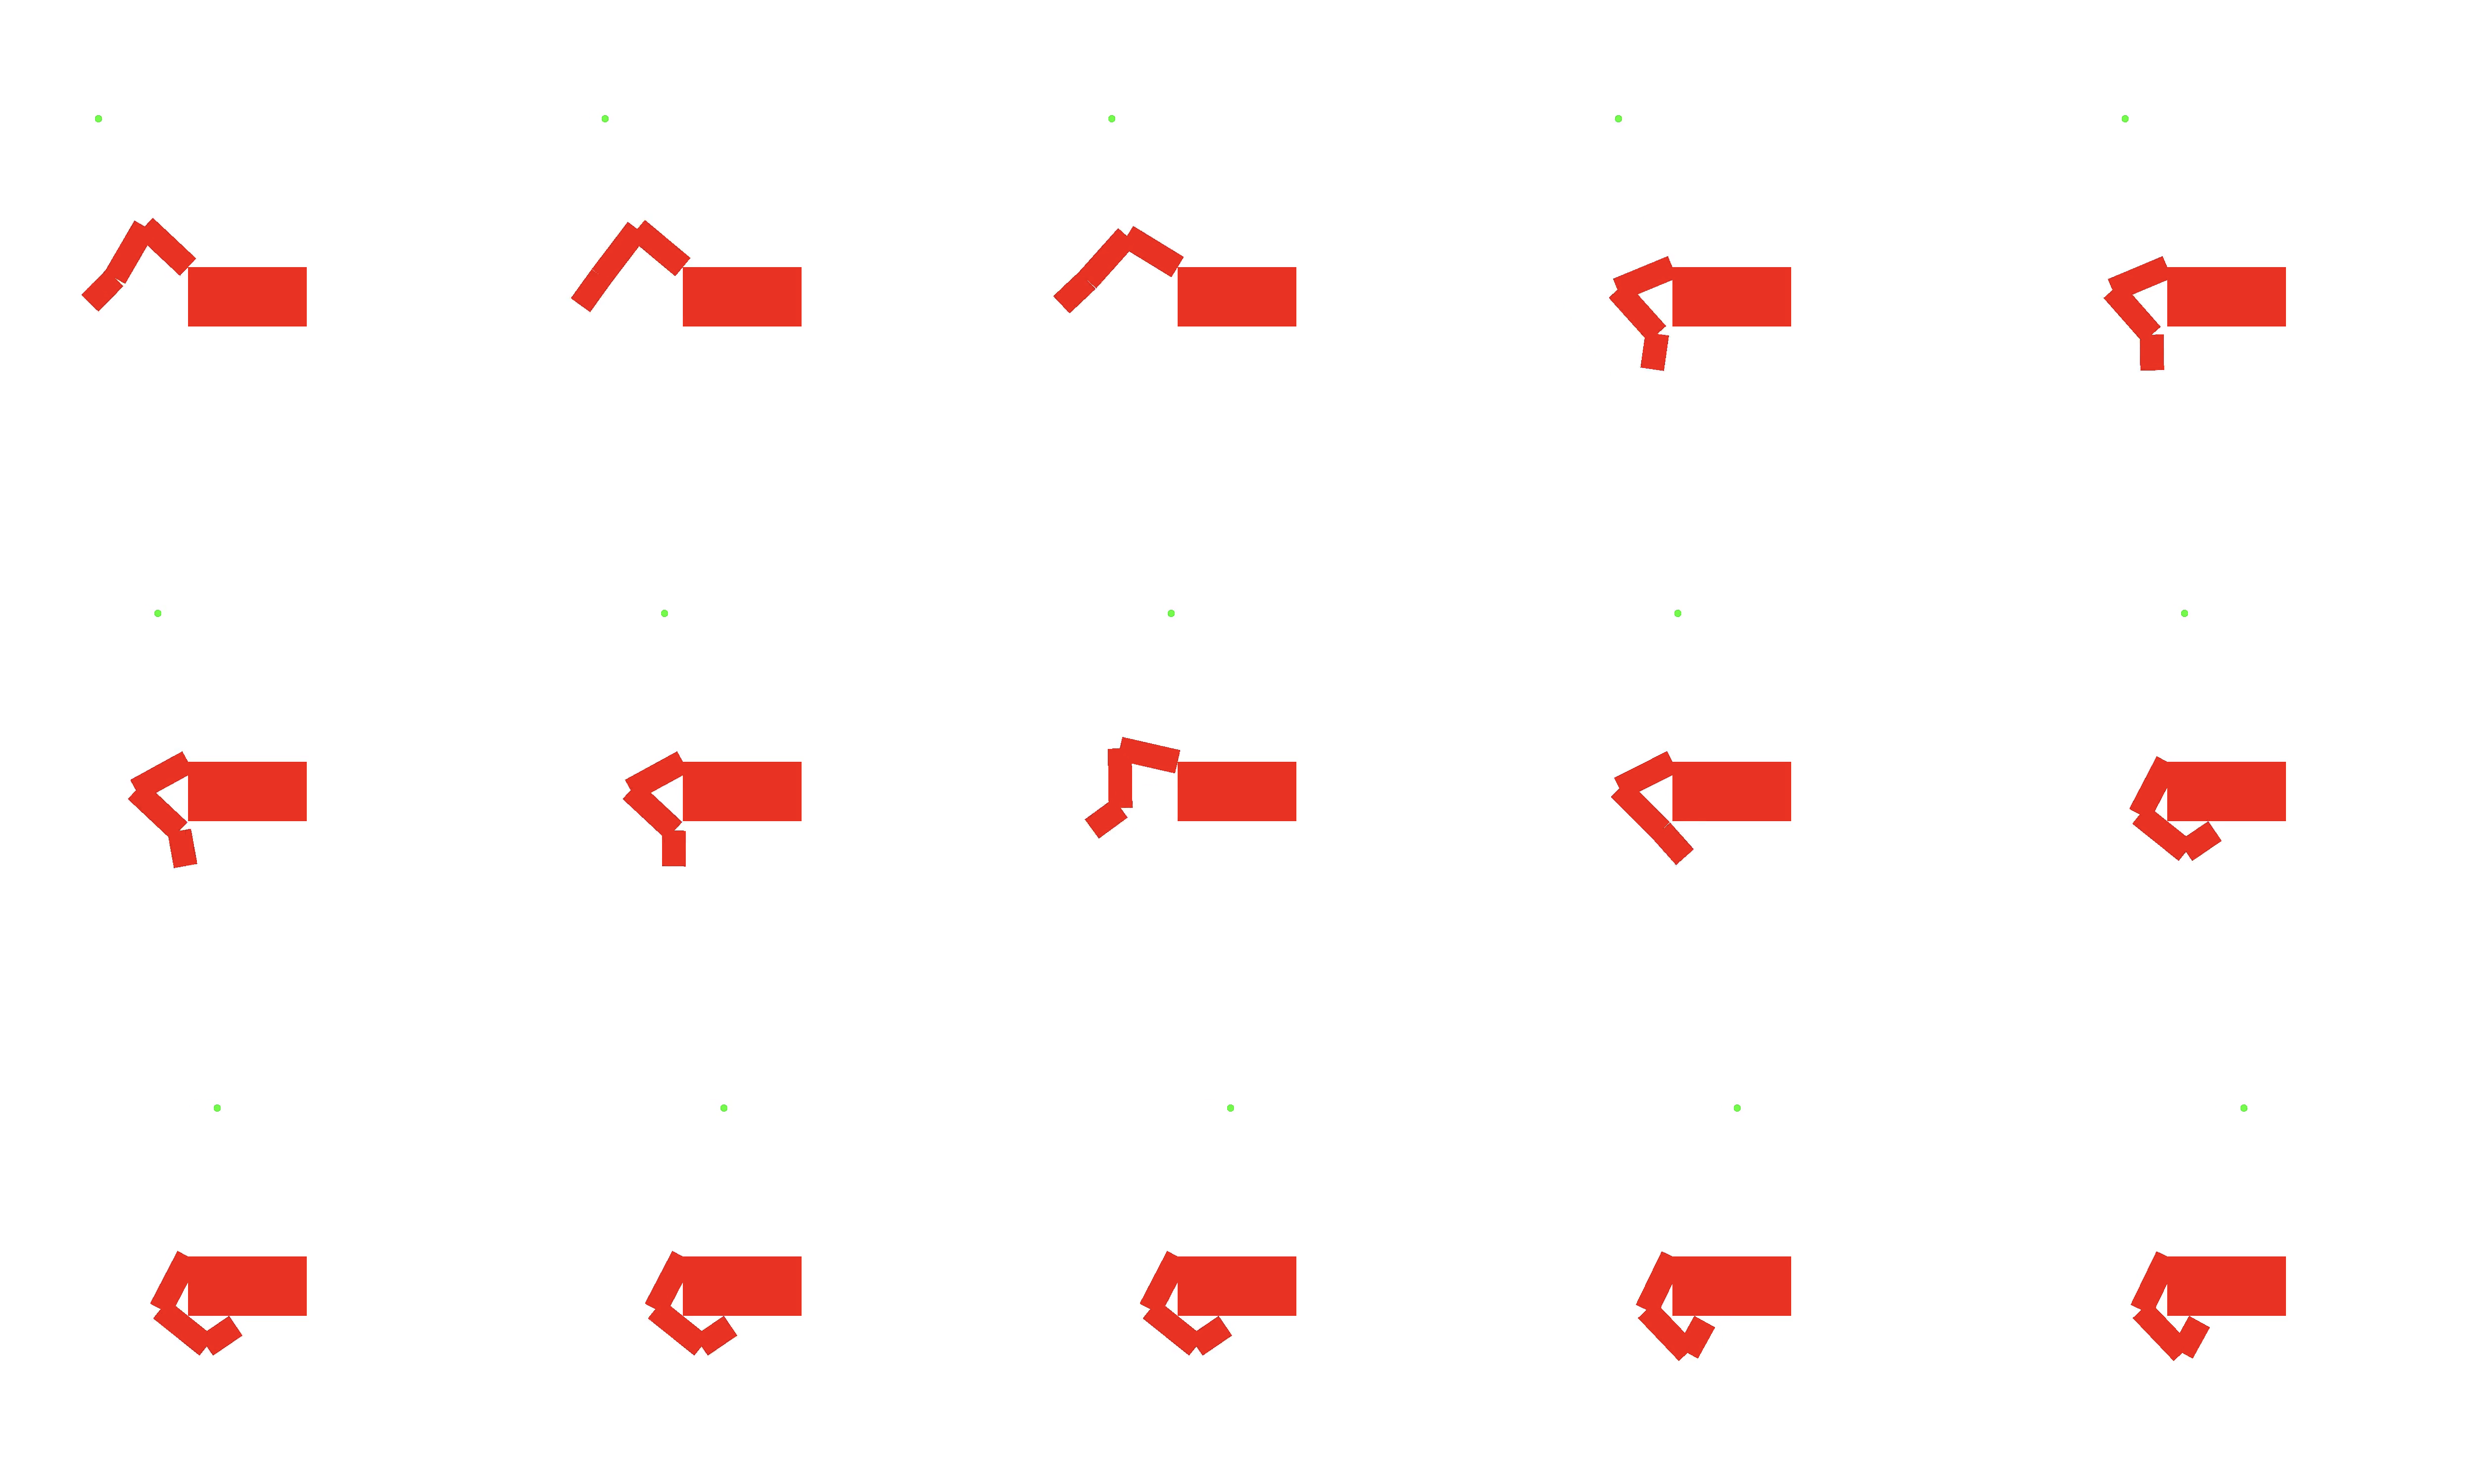
\includegraphics[width=1\textwidth]{figures/frames/frames_005.png}
      \caption{Control of a pigeon model with the body speed of 1 trained on $r_{fifty\_fifty}$}
      \label{fig:fifty_fifty_body_speed_1}
  \end{figure}


% summary of the results
  % 1.
  % 2.

  % 3. head wiggles relatively in the same position

  %\chapter{Analysis}
% variance between the two trajectories/paths

  \chapter{Discussion}
% "results indicate that..."
  % Examining the trajectory of each of the pigeon models' heads,
  % the resulting behavior exhibited by the pigeon model with a fixed body, whose deep reinforcement learning controller was trained on $r_{fifty\_fifty}$, indicate that the combination of visual stabilization and motion parallax are sufficient to generate a behavior that fixes the position of the head, resembling the hold phase in pigeons.

  % On the other hand, the resulting behavior exhibited by the pigeon model with body speed 1, whose deep reinforcement learning controller was trained on the same reward function, indicate that the 2 functionalities are insufficient to produce head-bobbing behaviors in moving bodies during forward locomotion, as he pigeon model did not need to periodically thrust its head forward to maximize Davies' equation depicting motion parallax between objects.

  % Such results indicate that visual stabilization with retinal cells capable of detecting movement in all directions is enough to maximize the sum of external objects' angular velocities within the retina.
    % Examining Davies' equation \ref{davies_motion_parallax}, it can be hypothesized that
    % reinforcement learning controllers trained on reward function that reflect such function would only reproduce head-bobbing behaviors
    % when all objects within the retina are globally static, since the equation does not account for the objects' velocities.
    % Since the external objects in our experiment had objects moving forwards and backwards, such may have automatically increased the reward function depicting Davies' equation of motion parallax per timestep.


% may need a state machine-like mechanism for replication of head-bob
  % composed of the "hold phase" state and the "thrust phase" state
% hierarchical control system
  % hierarchical reinforcement learning should be used for modeling the control system with this hypothesis
% indicates that a hierarchical control system is embedded in pigeons' neurology.
% pattern generating module or functionality, such as central pattern generators seen in the spinal cortex

% head goes downwards during forward locomotion
% lack of muscular strain penalty?

% needs higher details, such as an addition of muscular physics, and progression in incremental modeling
% muscular simulation and their placements upon the skeletal model may lead to more stabilization (cite Geijtenbeek)

  %\input{futurework.tex}


  % Acknowledgements
  \acknowledgements
  Lorem ipsum dolor sit amet, consectetur adipiscing elit. In efficitur porta augue, at interdum nunc lobortis at. Morbi feugiat facilisis justo, vitae maximus dolor. Cras convallis at elit in porta. Fusce lobortis tortor nibh, quis imperdiet arcu luctus quis. Mauris imperdiet urna eu mauris aliquet, vitae tincidunt orci dapibus. Vestibulum convallis elit ut velit accumsan cursus. Pellentesque lacus lacus, blandit eu felis vitae, pellentesque dignissim est.



  % Reference
  \newpage
  %\reference
  \nocite{*}
  %\nocite{*} %Use if you want to list everything listed in bibtex, if not comment it out

  %Bibliography
  %\bibliographystyle{abbrv}

  %ACM SIGCHI Style
  \bibliographystyle{acm-sigchi}
  \bibliography{ref}

  % Appendix
  \appendix
  \section{OpenAI Gym for Simplified Model of Pigeons' Head Control}
% written in Python

% reference to OpenAI Gym library site or paper

\subsection{Usage}
\begin{lstlisting}
PigeonEnv3Joints(self, body_speed = 0,
                 reward_code = "head_stable_manual_reposition",
                 max_offset = 0.5)
\end{lstlisting}
\begin{itemize}
    \item \lstinline|body_speed| indicates the speed in which the pigeon model's body moves.

    \item Each of the following \lstinline|reward_code| are assigned to their respective reward functions.
        \begin{itemize}
          \item \lstinline|"head_stable_manual_reposition"|
              \begin{description}
                  \item Implementation of $r_{head\_stable\_manual\_reposition}$
              \end{description}
          \item \lstinline|"head_stable_manual_reposition_strict_angle"|
              \begin{description}
                  \item Implementation of $r_{head\_stable\_manual\_reposition\_strict\_angle}$
              \end{description}
        \end{itemize}
    \item \lstinline|max_offset| indicates the $max\_offset$ for each reward function to reference.
\end{itemize}

\begin{lstlisting}
PigeonRetinalEnv(self,
                 body_speed = 0,
                 reward_code = "motion_parallax")
\end{lstlisting}

Parallel to \lstinline|PigeonEnv3Joints|, each of the following \lstinline|reward_code| are assigned to their respective reward functions.
\begin{itemize}
  \item \lstinline|"retinal_stabilization"|
      \begin{description}
          \item Implementation of $r_{head\_stabilize}$
          \item Depicts the preliminary hypothesis regarding the functionality of retinal stabilization during the hold phase.
      \end{description}
  \item \lstinline|"motion_parallax"|
      \begin{description}
          \item Implementation of $r_{motion\_parallax}$
          \item Depicts the preliminary hypothesis regarding the functionality of motion parallax induced depth perception during the thrust phase.
      \end{description}
  \item \lstinline|"fifty_fifty"|
      \begin{itemize}
          \item Implementation of $r_{head\_stable\_manual\_reposition\_strict\_angle}$
          \item Sum of rewards produced by  \lstinline|"retinal_stabilization"| and \lstinline|"motion_parallax"|
      \end{itemize}
\end{itemize}

% dependencies
\subsection{Dependencies (Anaconda YAML File)}
The listed versions are recommendations and not strictly necessary for replication
\begin{lstlisting}
name: pigeon-env
channels:
  - conda-forge
  - defaults
dependencies:
  - bzip2=1.0.8=h0d85af4_4
  - ca-certificates=2021.10.8=h033912b_0
  - certifi=2016.9.26=py36_0
  - ffmpeg=4.3.2=h4dad6da_0
  - freetype=2.10.4=h4cff582_1
  - future=0.18.2=py36h79c6626_3
  - gettext=0.19.8.1=h7937167_1005
  - gmp=6.2.1=h2e338ed_0
  - gnutls=3.6.13=h756fd2b_1
  - lame=3.100=h35c211d_1001
  - libcxx=12.0.0=h2f01273_0
  - libffi=3.3=hb1e8313_2
  - libiconv=1.16=haf1e3a3_0
  - libpng=1.6.37=h7cec526_2
  - ncurses=6.3=hca72f7f_2
  - nettle=3.6=hedd7734_0
  - openh264=2.1.1=hfd3ada9_0
  - openssl=1.1.1l=h0d85af4_0
  - pip=21.2.2=py36hecd8cb5_0
  - pybox2d=2.3.10=py36hefe7e0e_1
  - pyglet=1.5.16=py36h79c6626_0
  - python=3.6.13=h88f2d9e_0
  - python_abi=3.6=2_cp36m
  - readline=8.1.2=hca72f7f_1
  - setuptools=58.0.4=py36hecd8cb5_0
  - sqlite=3.37.0=h707629a_0
  - tk=8.6.11=h7bc2e8c_0
  - wheel=0.37.1=pyhd3eb1b0_0
  - x264=1!161.3030=h0d85af4_1
  - xz=5.2.5=h1de35cc_0
  - zlib=1.2.11=h4dc903c_4
  - pip:
    - cloudpickle==2.0.0
    - gym==0.21.0
    - importlib-metadata==4.8.3
    - numpy==1.19.5
    - typing-extensions==4.0.1
    - zipp==3.6.0
\end{lstlisting}

  % \chapter{Appendix}
\section{OpenAI Gym for Simplified Model of Pigeons' Head Control}

% reference to OpenAI Gym library site or paper
% reward function names


\subsection{Manually Defined Head Trajectory (Baseline)}
% Python code as of 01-08-22
\begin{lstlisting}
from Box2D import *
import gym
from gym import spaces

from math import sin, pi, sqrt
import numpy as np
from copy import copy, deepcopy

# anatomical variables ("macros")
BODY_WIDTH = 10
BODY_HEIGHT = 5

LIMB_WIDTH = 5
LIMB_HEIGHT = 2

HEAD_WIDTH = 3

ANGLE_FREEDOM = 0.6

# control variables/macros
MAX_JOINT_TORQUE = 200 #70
MAX_JOINT_SPEED = 5 #10
VELOCITY_WEIGHT = 1.0 #0.9
LIMB_DENSITY = 0.1 ** 3
LIMB_FRICTION = 5

VIEWPORT_SCALE = 6.0
FPS = 60

HEAD_OFFSET_X = 10
HEAD_OFFSET_Y = 2

class PigeonEnv3Joints(gym.Env):
    metadata = {"render.modes": ["human", "rgb_array"], "video.frames_per_second": FPS}

    def __init__(self,
                 body_speed = 0,
                 reward_code = "head_stable_manual_reposition",
                 max_offset = 0.5):
        """
        Action and Observation space
        """

        # 3-dim joints' torque ratios
        self.action_space = spaces.Box(
            np.array([-1.0] * 3).astype(np.float32),
            np.array([1.0] * 3).astype(np.float32),
        )
        # 2-dim head location;
        # 1-dim head angle;
        # 3x2-dim joint angle and angular velocity;
        # 1-dim x-axis of the body
        # [NEW] 2-dim target head location
        high = np.array([np.inf] * 12).astype(np.float32) # formally 10
        self.observation_space = spaces.Box(-high, high)

        """
        Box2D Pigeon Model Params and Initialization
        """
        self.world = b2World()                          # remove in Framework
        self.body = None
        self.joints = []
        self.head = None
        self.bodyRef = [] # for destruction
        self.body_speed = body_speed
        self._pigeon_model()

        """
        Box2D Simulation Params
        """
        self.timeStep = 1.0 / FPS
        self.vel_iters, self.pos_iters = 10, 10

        self.viewer = None

        """
        Assigning a Reward Function
        """
        self._assign_reward_func(reward_code, max_offset)

    """
    Define Reward Function and Necessary Parameters
    """
    def _assign_reward_func(self, reward_code, max_offset):
        if "head_stable_manual_reposition" in reward_code:
            self.max_offset = max_offset

            self.relative_repositioned_head_target_location = np.array(self.head.position) - np.array([0, HEAD_OFFSET_Y])
            self.head_target_location = self.relative_repositioned_head_target_location + np.array(self.body.position)
            self.head_target_angle = self.head.angle
            self.reward_function = self._head_stable_manual_reposition

            if "strict_angle" in reward_code:
                self.reward_function = self._head_stable_manual_reposition_strict_angle

        else:
            raise ValueError("Unknown reward_code")

    """
    Box2D Pigeon Model
    """
    def _pigeon_model(self):
        # params
        body_anchor = np.array([float(-BODY_WIDTH), float(BODY_HEIGHT)])
        limb_width_cos = LIMB_WIDTH / sqrt(2)

        self.bodyRef = []
        # body definition
        self.body = self.world.CreateKinematicBody(
            position = (0, 0),
            shapes = b2PolygonShape(box = (BODY_WIDTH, BODY_HEIGHT)), # x2 in direct shapes def
            linearVelocity = (-self.body_speed, 0),
            angularVelocity = 0,
            )
        self.bodyRef.append(self.body)

        # neck as limbs + joints definition
        self.joints = []
        current_center = deepcopy(body_anchor)
        current_anchor = deepcopy(body_anchor)
        offset = np.array([-limb_width_cos, limb_width_cos])
        prev_limb_ref = self.body
        for i in range(2):
            if i == 0:
                current_center += offset

            else:
                current_center += offset * 2
                current_anchor += offset * 2

            tmp_limb = self.world.CreateDynamicBody(
                position = (current_center[0], current_center[1]),
                fixtures = b2FixtureDef(density = LIMB_DENSITY,
                                        friction = LIMB_FRICTION,
                                        restitution = 0.0,
                                        shape = b2PolygonShape(
                                            box = (LIMB_WIDTH, LIMB_HEIGHT)),
                                        ),
                angle = -pi / 4
            )
            self.bodyRef.append(tmp_limb)

            tmp_joint = self.world.CreateRevoluteJoint(
                bodyA = prev_limb_ref,
                bodyB = tmp_limb,
                anchor = current_anchor,
                lowerAngle = -ANGLE_FREEDOM * b2_pi, # -90 degrees
                upperAngle = ANGLE_FREEDOM * b2_pi,  #  90 degrees
                enableLimit = True,
                maxMotorTorque = MAX_JOINT_TORQUE,
                motorSpeed = 0.0,
                enableMotor = True,
            )

            self.joints.append(tmp_joint)
            prev_limb_ref = tmp_limb

        # head def + joints
        current_center += offset
        current_anchor += offset * 2
        self.head = self.world.CreateDynamicBody(
            position = (current_center[0] - HEAD_WIDTH, current_center[1]),
            fixtures = b2FixtureDef(density = LIMB_DENSITY,
                                    friction = LIMB_FRICTION,
                                    restitution = 0.0,
                                    shape = b2PolygonShape(
                                        box = (HEAD_WIDTH, LIMB_HEIGHT)),
                                    ),
        )
        self.bodyRef.append(self.head)

        head_joint = self.world.CreateRevoluteJoint(
            bodyA = prev_limb_ref,
            bodyB = self.head,
            anchor = current_anchor,
            lowerAngle = -ANGLE_FREEDOM * b2_pi, # -90 degrees
            upperAngle = ANGLE_FREEDOM * b2_pi,  #  90 degrees
            enableLimit = True,
            maxMotorTorque = MAX_JOINT_TORQUE,
            motorSpeed = 0.0,
            enableMotor = True,
        )
        self.joints.append(head_joint)

        # head tracking
        self.head_prev_pos = np.array(self.head.position)
        self.head_prev_ang = self.head.angle

    def _destroy(self):
        for body in self.bodyRef:
            # all associated joints are destroyed implicitly
            self.world.DestroyBody(body)

    def _get_obs(self):
        # (self.head{relative}, self.joints -> obs) operation
        obs = np.array(self.head.position) - np.array(self.body.position)
        obs = np.concatenate((obs, self.head.angle), axis = None)
        for i in range(len(self.joints)):
            obs = np.concatenate((obs, self.joints[i].angle), axis = None)
            obs = np.concatenate((obs, self.joints[i].speed), axis = None)
        obs = np.concatenate((obs, self.body.position[0]), axis = None)

        # complement a target position
        obs = np.concatenate((obs, self.head_target_location - np.array(self.body.position)),
                              axis = None)

        obs = np.float32(obs)
        assert self.observation_space.contains(obs)
        return obs

    def reset(self):
        self._destroy()
        self._pigeon_model()
        return self._get_obs()

    def _head_target_reposition_mechanism(self):
        # detect whether the target head position is behind the body edge or not
        if self.head_target_location[0] > self.body.position[0] - float(BODY_WIDTH + HEAD_OFFSET_X):
            self.head_target_location = np.array(self.body.position) + \
                self.relative_repositioned_head_target_location

        head_dif_loc = np.linalg.norm(np.array(self.head.position) - \
                self.head_target_location)
        head_dif_ang = abs(self.head.angle - self.head_target_angle)
        return head_dif_loc, head_dif_ang

    """
    Modular Reward Functions
    """
    def _head_stable_manual_reposition(self):
        # This method is separated from step(), since there are variables used
        # that are only defined in with this strain of reward functions
        head_dif_loc, head_dif_ang = self._head_target_reposition_mechanism()

        reward = 0
        # threshold reward function with static offset
        if head_dif_loc < self.max_offset:
            reward += 1 - head_dif_loc/self.max_offset

            if head_dif_ang < np.pi / 6: # 30 deg
                reward += 1 - head_dif_ang/ np.pi

        return reward

    def _head_stable_manual_reposition_strict_angle(self):
        head_dif_loc, head_dif_ang = self._head_target_reposition_mechanism()

        reward = 0
        # threshold reward function with static offset
        if head_dif_loc < self.max_offset:
            if head_dif_ang < np.pi / 6: # 30 deg
                reward += 1 - head_dif_ang/ np.pi

        return reward

    def step(self, action):
        assert self.action_space.contains(action)
        # self.world.Step(self.timeStep, self.vel_iters, self.pos_iters)
        # Framework handles this differently
        # Referenced bipedal_walker
        # self.world.Step(1.0 / 50, 6 * 30, 2 * 30)
        self.world.Step(1.0 / FPS, self.vel_iters, self.pos_iters)
        obs = self._get_obs()

        # MOTOR CONTROL
        for i in range(len(self.joints)):
            # Copied from bipedal_walker
            self.joints[i].motorSpeed = float(MAX_JOINT_SPEED * (VELOCITY_WEIGHT ** i) * np.sign(action[i]))
            self.joints[i].maxMotorTorque = float(
                MAX_JOINT_TORQUE * np.clip(np.abs(action[i]), 0, 1)
            )

        reward = self.reward_function()

        done = False
        info = {}
        return obs, reward, done, info

    def render(self, mode = "human"):
        from gym.envs.classic_control import rendering
        if self.viewer is None:
            self.viewer = rendering.Viewer(500, 500)

            # Set ORIGIN POINT relative to camera
            self.camera_trans = b2Vec2(-250, -200) \
            + VIEWPORT_SCALE * self.bodyRef[0].position # camera moves with body

            ## Needs head_stable_manual_reposition reward function to execute
            try:
                # init visualize max_offset
                render_target_area = rendering.make_circle( \
                    radius=VIEWPORT_SCALE * self.max_offset,
                    res=30,
                    filled=True)
                target_translate = rendering.Transform(
                    translation = VIEWPORT_SCALE * self.head_target_location - self.camera_trans,
                    rotation = 0.0,
                    scale = VIEWPORT_SCALE * np.ones(2)
                )
                render_target_area.add_attr(self.target_translate)
                render_target_area.set_color(0.0, 1.0, 0.0)
                self.viewer.add_geom(render_target_area)
            except:
                pass

            # init translation and rotation for each limb
            self.render_polygon_list = []
            self.render_polygon_rotate_list = []
            self.render_polygon_translate_list = []
            for body in self.bodyRef:
                polygon = rendering.FilledPolygon(
                    body.fixtures[0].shape.vertices
                )
                rotate = rendering.Transform(
                    translation = (0.0, 0.0),
                    rotation = body.angle,
                )
                translate = rendering.Transform(
                    translation = VIEWPORT_SCALE * body.position - self.camera_trans,
                    rotation = 0.0,
                    scale = VIEWPORT_SCALE * np.ones(2)
                )
                polygon.set_color(1.0, 0.0, 0.0)
                polygon.add_attr(rotate)
                polygon.add_attr(translate)
                self.render_polygon_list.append(polygon)
                self.render_polygon_rotate_list.append(rotate)
                self.render_polygon_translate_list.append(translate)
                self.viewer.add_geom(polygon)

        # Update ORIGIN POINT relative to camera
        self.camera_trans = b2Vec2(-250, -200) \
        + VIEWPORT_SCALE * self.bodyRef[0].position # camera moves with body

        ## Needs head_stable_manual_reposition reward function to execute
        try:
            # update max_offset shape translation
            new_target_translate = VIEWPORT_SCALE * self.head_target_location - self.camera_trans
            self.target_translate.set_translation(new_target_translate[0], new_target_translate[1])
        except:
            pass

        # update body rotation and translation
        for i, body in enumerate(self.bodyRef):
            self.render_polygon_rotate_list[i].set_rotation(body.angle)
            new_body_translate = VIEWPORT_SCALE * body.position - self.camera_trans
            self.render_polygon_translate_list[i].set_translation(new_body_translate[0], new_body_translate[1])

        return self.viewer.render(return_rgb_array = mode == "rgb_array")

    def close(self):
        # self._destroy()
        # self.world = None

        if self.viewer:
            self.viewer.close()
            self.viewer = None
\end{lstlisting}

  \subsection{Pigeons' Head Control Based on Retinal Inputs}
% Python code as of 01-15-22
\begin{lstlisting}
import PigeonEnv3Joints, VIEWPORT_SCALE
import numpy as np
import gym
from gym import spaces

class PigeonRetinalEnv(PigeonEnv3Joints):

    def __init__(self,
                 body_speed = 0,
                 reward_code = "motion_parallax"):

        """
        Object Location Init (2D Tensor)
        """
        self.objects_position = np.array([[-30.0, 30.0],
                                          [-30.0, 60.0],
                                          [-60.0, 30.0],])
        self.objects_velocity = np.array([[0.0, 0.0],
                                          [1.0, 0.0],
                                          [-1.0, 0.0],])

        """
        Init based on superclass
        Reward function is defined here
        """
        super().__init__(body_speed, reward_code)

        """
        Redefining Observation space
        """
        # 2-dim head location;
        # 1-dim head angle;
        # 3x2-dim joint angle and angular velocity;
        # 1-dim x-axis of the body
        high = np.array([np.inf] * 10).astype(np.float32) # formally 10
        self.observation_space = spaces.Box(-high, high)


    """
    Retinal coords (angles); Within [-np.pi, np.pi]
    """
    def _get_retinal(self, object_position):
        # normalized direction of object from head
        object_direction = object_position - np.array(self.head.position)
        object_direction = object_direction / np.linalg.norm(object_direction)

        sign = np.ones(object_direction.shape[0])
        for i in range(sign.size):
            # is the object above or below the head?
            if object_direction[i][1] < 0:
                sign[i] = -1

        # calculate COSINE angle of object relative to head (positive if above, negative if below)
        # cosine_angle is of size [num_objects,]
        cosine_angle = sign * np.arccos( \
            np.dot(object_direction, np.array([-1.0, 0.0])))

        # differnce in angle between the head angle and sine_angle of head
        relative_angle = cosine_angle + self.head.angle

        # relative_angle should be within [-np.pi, np.pi]
        for i in range(relative_angle.shape[0]):
            if relative_angle[i] < -np.pi:
                k = 1
                while relative_angle[i] < (k + 1) * -np.pi:
                    k += 1
                relative_angle[i] = relative_angle[i] + 2 * np.pi * ((k + 1) // 2)

            elif relative_angle[i] > np.pi:
                k = 1
                while relative_angle[i] > (k + 1) * np.pi:
                    k += 1
                relative_angle[i] = relative_angle[i] - 2 * np.pi * ((k + 1) // 2)

        return relative_angle

    def _get_angular_velocity(self, prev_ang, current_ang):
        angle_velocity = current_ang - prev_ang
        angle_speed = np.absolute(angle_velocity)
        for i in range(angle_velocity.size):
            if angle_speed[i] > np.pi:
                angle_velocity[i] = 2 * np.pi - angle_velocity[i]
            elif angle_speed[i] < -np.pi:
                angle_velocity[i] = 2 * np.pi + angle_velocity[i]
            else:
                pass
        return angle_velocity

    """
    Defining Reward Functions
    """
    def _assign_reward_func(self, reward_code, max_offset = None):
        self.prev_angle = self._get_retinal(self.objects_position)
        if "motion_parallax" in reward_code:
            self.reward_function = self._motion_parallax
        elif "retinal_stabilization" in reward_code:
            self.reward_function = self._retinal_stabilization
        elif "fifty_fifty" in reward_code:
            self.reward_function = self._fifty_fifty
        else:
            raise ValueError("Unknown reward_code")

    def _motion_parallax(self):
        current_angle = self._get_retinal(self.objects_position)

        parallax_velocities = \
            self._get_angular_velocity(current_angle, self.prev_angle)

        reward = 0
        # sum of motion parallax magnitudes
        for i in range(parallax_velocities.size):
            for j in range(i, parallax_velocities.size):
                reward += np.abs(parallax_velocities[i] - parallax_velocities[j])
            # reward += parallax_velocities[i]
        return reward

    def _retinal_stabilization(self):
        reward = 0
        current_angle = self._get_retinal(self.objects_position)
        relative_speeds = \
            np.absolute(self._get_angular_velocity(current_angle, self.prev_angle))
        reward -= np.sum(relative_speeds)
        return reward

    def _fifty_fifty(self):
        reward = 0
        reward += self._retinal_stabilization()
        reward += self._motion_parallax()
        return reward

    def _get_obs(self):
        # (self.head{relative}, self.joints -> obs) operation
        obs = np.array(self.head.position) - np.array(self.body.position)
        obs = np.concatenate((obs, self.head.angle), axis = None)
        for i in range(len(self.joints)):
            obs = np.concatenate((obs, self.joints[i].angle), axis = None)
            obs = np.concatenate((obs, self.joints[i].speed), axis = None)
        obs = np.concatenate((obs, self.body.position[0]), axis = None)
        obs = np.float32(obs)
        assert self.observation_space.contains(obs)
        return obs

    def step(self, action):
        self.prev_angle = self._get_retinal(self.objects_position)
        # alter object
        self.objects_position += self.objects_velocity
        return super().step(action)

    def render(self, mode = "human"):
        from gym.envs.classic_control import rendering
        if self.viewer is None:
            self.render_objects_list = None
            self.render_objects_translate_list = None

        super().render(mode)
        # initialize object rendering pointers
        if self.render_objects_list is None:
            self.render_objects_list = []
            self.render_objects_translate_list = []
            for i in range(self.objects_position.shape[0]):
                object_render_instance = rendering.make_circle( \
                    radius=0.6,
                    res=30,
                    filled=True)
                object_render_instance_translate = rendering.Transform(
                    translation = VIEWPORT_SCALE * \
                        (self.objects_position[i] - self.camera_trans),
                    rotation = 0.0,
                    scale = VIEWPORT_SCALE * np.ones(2)
                )
                object_render_instance.add_attr(object_render_instance_translate)
                object_render_instance.set_color(0.0, 1.0, 0.0)
                self.render_objects_list.append(object_render_instance)
                self.render_objects_translate_list.append(object_render_instance_translate)
                self.viewer.add_geom(object_render_instance)

        # update object translation
        new_object_translate = VIEWPORT_SCALE * self.objects_position - self.camera_trans
        for i in range(self.objects_position.shape[0]):
            self.render_objects_translate_list[i].set_translation( \
                new_object_translate[i][0], new_object_translate[i][1])

        return self.viewer.render(return_rgb_array = mode == "rgb_array")
\end{lstlisting}

  \newpage
  \section{Hyperparameters for Soft Actor Critic Training}
\subsection{}
% SAC training workflow
  % \cite{haarnoja2018soft}
  \begin{figure}[H]
      \centering
      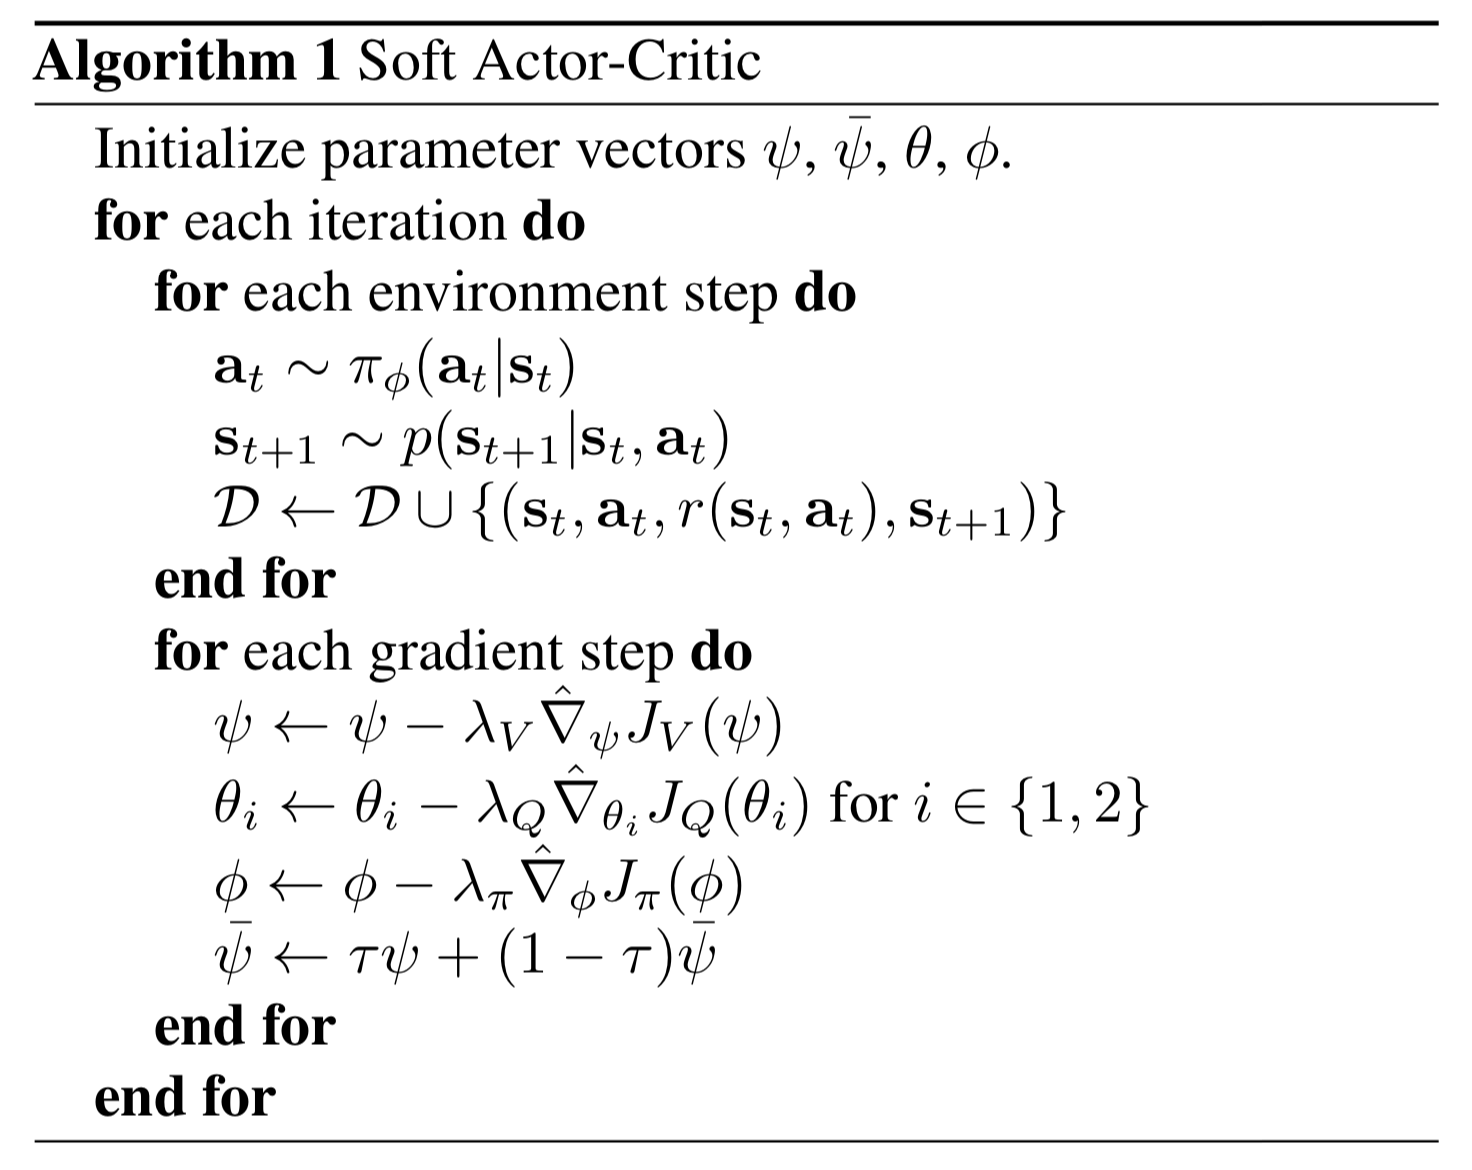
\includegraphics[width=1\textwidth]{figures/external/sac_algorithm.png}
      \caption{Soft Actor Critic algorithm as shown in \cite{haarnoja2018soft}}
      \label{fig:}
  \end{figure}

% batch training
% hidden layer size 256
% epochs 3000

% timesteps per training loop 1000
% param update per training loop 1000
% batch size 256
% replay_buffer_size=int(1E6),

% layer_size=256,
%     replay_buffer_size=int(1E6),
%     algorithm_kwargs=dict(
%         num_epochs=3000,
%         num_eval_steps_per_epoch=5000, % this is for evaluation
%         num_trains_per_train_loop=1000,
%         num_expl_steps_per_train_loop=1000,
%           min_num_steps_before_training=1000,
%           max_path_length=1000,
%         batch_size=256,
%     ),
%     trainer_kwargs=dict(
%         discount=0.99,
%         soft_target_tau=5e-3,
%         target_update_period=1,
%         policy_lr=3E-4,
%         qf_lr=3E-4,
%         reward_scale=1,
%         use_automatic_entropy_tuning=True,
%     ),

  % NO Appendix 3! Do NOT include raw trajectory data!
\end{document}
